\chapter{Mendix} \label{ch:mendix}
    Έχοντας πλέον μια καλή εικόνα για τον ορισμό του χαμηλού κώδικα και των Πλατφορμών Ανάπτυξης Λογισμικού σε Low-Code, στο παρόν κεφάλαιο, θα επικεντρωθούμε σε μια από αυτές τις πλατφόρμες, το Mendix, η οποία αποτέλεσε το βασικό εργαλείο για την υλοποίηση της εφαρμογής που αναπτύχθηκε στο πλαίσιο αυτής της διπλωματικής εργασίας.

    Σε αυτό το κεφάλαιο, θα περιγραφεί το γραφικό περιβάλλον του Mendix Studio Pro, και θα αναλυθεί η δομή μιας εφαρμογής που αναπτύσσεται στο Mendix. Θα περιγραφούν έννοιες όπως τα modules, τα έγγραφα, τα widgets, οι σελίδες, τα microflows, τα domain models και άλλα. Ο στόχος είναι να κατανοηθεί πλήρως η δομή μιας εφαρμογής στο Mendix, πριν προχωρήσουμε στη διαδικασία υλοποίησης στο επόμενο κεφάλαιο.

    \section{Τι είναι το Mendix;}
        Το Mendix αποτελεί μία από τις πιο διαδεδομένες πλατφόρμες ανάπτυξης λογισμικού που βασίζεται σε χαμηλό κώδικα. Ιδρύθηκε το 2005 στο Ρότερνταμ της Ολλανδίας με στόχο να παρέχει στους επιχειρηματίες και τους οργανισμούς τη δυνατότητα να αναπτύσσουν, να προσαρμόζουν και να διαχειρίζονται εφαρμογές αποδοτικά με χαμηλό κόστος. Το Mendix περιλαμβάνει όλα τα οφέλη και τα χαρακτηριστικά των LCDP που έχουν περιγραφεί στην ενότητα \ref{sec:LCDP}, συμπεριλαμβάνοντας γραφικό περιβάλλον με WYSIWYG GUI σχεδιαστή, drag-and-drop εργαλεία και έτοιμες βιβλιοθήκες, τη χρήση domain models, το εύκολο deployment της εφαρμογής στο cloud, version control μέσω Git, συνεργασία χρησιμοποιώντας Agile μεθοδολογία και άλλα.

        Το 2018, το Mendix εξαγοράστηκε από τη Siemens, τη μεγαλύτερη βιομηχανική κατασκευαστική εταιρεία στην Ευρώπη, γεγονός που επέφερε σημαντικές εξελίξεις στην πλατφόρμα. Η συγχώνευση αυτή επέτρεψε την ενσωμάτωση προηγμένων βιομηχανικών και IoT (Internet of Things) λύσεων, ενισχύοντας τη θέση του Mendix στην αγορά των λογισμικών σχεδιασμένων για επιχειρήσεις. Έτσι, το Mendix συγκαταλέγεται στις πιο ισχυρές και ευέλικτες λύσεις στην αγορά του low-code προγραμματισμού, προσφέροντας αποτελεσματικότητα, ταχύτητα και καινοτομία στην ανάπτυξη λογισμικού, ενώ παράλληλα ενσωματώνει τις πιο σύγχρονες τεχνολογίες για να καλύψει τις ανάγκες επιχειρήσεων που επιθυμούν να παραμείνουν ανταγωνιστικές στην ψηφιακή εποχή \cite{LowCodeMendix}.

        Η Gartner, μια από τις μεγαλύτερες εταιρείες έρευνας και συμβουλευτικών υπηρεσιών στον κλάδο της τεχνολογίας, χαρακτηρίζει το Mendix ως ηγέτη στην αγορά των πλατφορμών ανάπτυξης λογισμικού για 8 συνεχόμενα χρόνια (εικόνα \ref{fig:GartnerQuadrant}). Η κατάταξη αυτή επιβεβαιώνει τη δυνατότητα του Mendix να παρέχει λύσεις υψηλής ποιότητας και αξίας στους πελάτες του, καθώς και την ικανότητά του να προσαρμόζεται στις ανάγκες της αγοράς και να προσφέρει συνεχώς καινοτόμες λύσεις \cite{mendixGartnerQuadrant}. Για αυτούς τους λόγους έχει προτιμηθεί για την υλοποίηση της εφαρμογής που θα παρουσιαστεί στο επόμενο κεφάλαιο.

            \begin{figure}[h!] \noindent \centering
                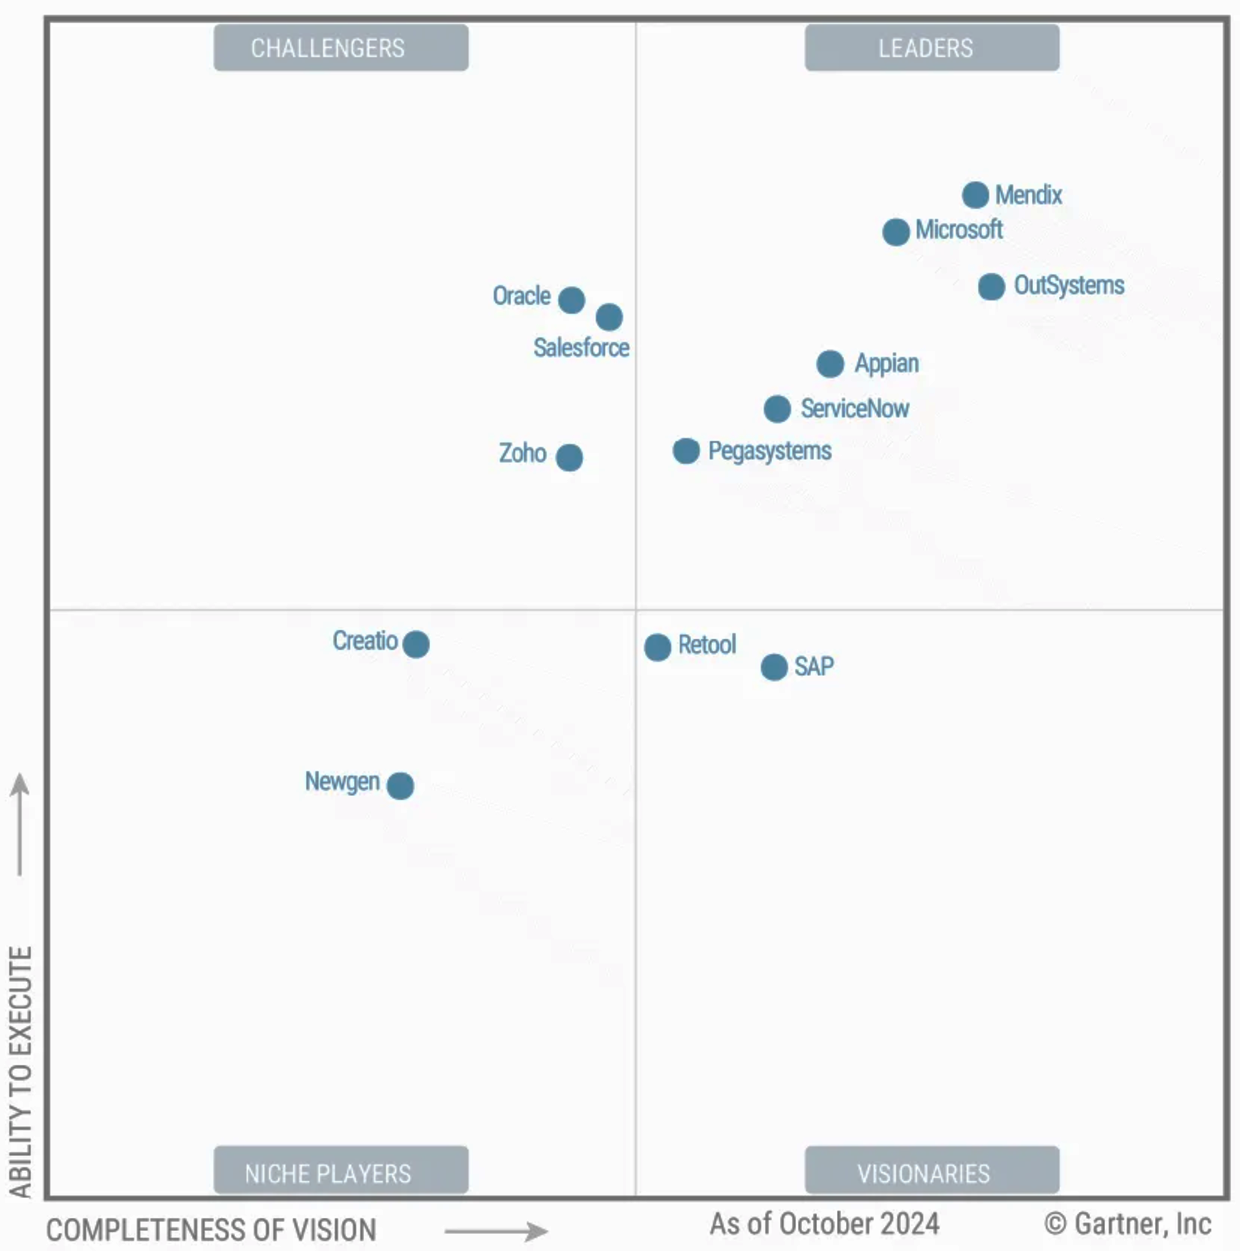
\includegraphics[width=0.5\textwidth]{GartnerQuadrant}
                \caption{\centering Τεταρτημόριο της Gartner με πλατφόρμες ανάπτυξης λογισμικού \cite{mendixGartnerQuadrant}}
                \label{fig:GartnerQuadrant}
            \end{figure}

    \section{Το Mendix Studio}
        Το Mendix Studio Pro αποτελεί το βασικό εργαλείο ανάπτυξης εφαρμογών της πλατφόρμας Mendix, προσφέροντας στους χρήστες τη δυνατότητα να δημιουργήσουν, να προσαρμόσουν, να δοκιμάσουν και να αναπτύξουν εφαρμογές.

        \begin{figure}[h!] \noindent \centering
            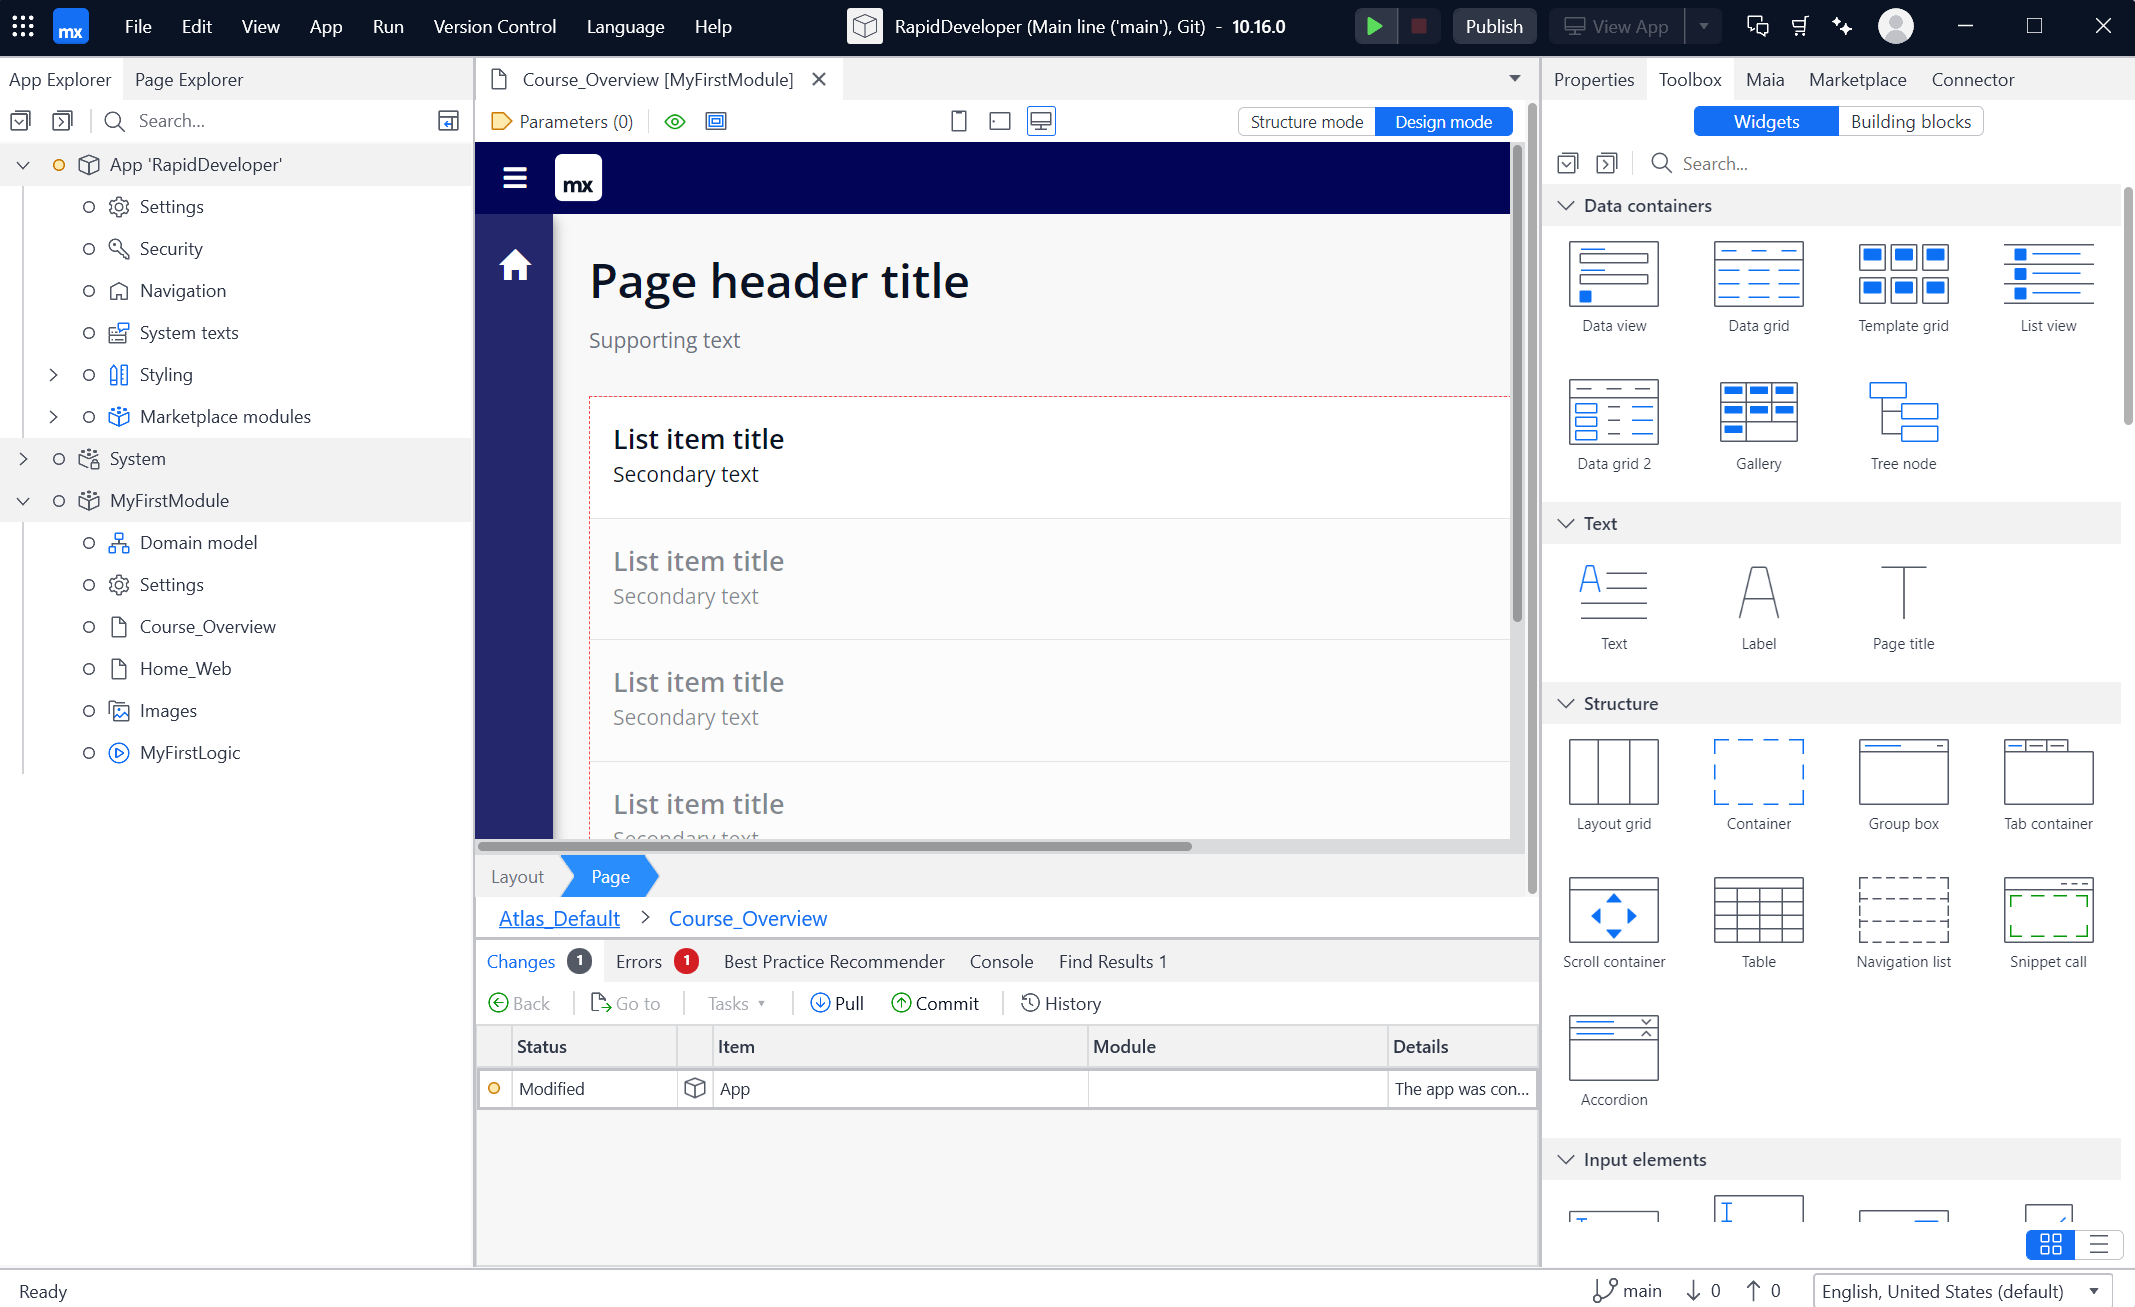
\includegraphics[width=\textwidth]{Mendix/MendixStudioOverlay}
            \caption{\centering Στιγμιότυπο του Mendix Studio Pro.}
            \label{fig:MendixStudioOverlay}
        \end{figure}

        \subsection{Περιβάλλον ανάπτυξης}
        Στο \ref{fig:MendixStudioOverlay} παρουσιάζεται το γραφικό περιβάλλον του Mendix Studio Pro με ανοιχτή την εφαρμογή RapidDeveloper\footnote{Η εφαρμογή RapidDeveloper δημιουργήθηκε ως αποτέλεσμα των μαθημάτων (crash courses) που προσφέρονται μέσω του Mendix Academy. Αυτά τα μαθήματα έχουν σχεδιαστεί για να παρέχουν στους χρήστες μια γρήγορη και πρακτική εισαγωγή στις βασικές δυνατότητες της πλατφόρμας Mendix, επιτρέποντάς τους να εξοικειωθούν με τη διαδικασία ανάπτυξης εφαρμογών σε περιβάλλον low-code.}.

        Μπορούμε να διαχωρίσουμε το γραφικό περιβάλλον σε τέσσερα μέρη. Η μαύρη μπάρα στο πάνω μέρος περιλαμβάνει το βασικό μενού της πλατφόρμας, το όνομα της εφαρμογής που αναπτύσσουμε, κουμπιά τα οποία επιτρέπουν είτε την τοπική εκτέλεση της εφαρμογής μέσω localhost ή τη διάθεσή της στο cloud (βλ. ενότητα \ref{sec:MendixDeployment}) και σύνδεσμοι που οδηγούν στο Mendix προφίλ του χρήστη, στο Marketplace κ.α.

        Στο κεντρικό τμήμα της οθόνης βρίσκεται το \textit{Working Area}, ένας WYSIWYG σχεδιαστής όπου μπορούμε να προβάλλουμε και να επεξεργαστούμε τις σελίδες της εφαρμογής μας. Μια σελίδα μπορεί να εμφανιστεί στο Working Area με διαφόρους τρόπους, οι οποίοι θα αναλυθούν στην ενότητα \ref{sec:MendixPageView}.

        Στην αριστερή πλευρά, εντοπίζουμε τον \textit{App Explorer}, ο οποίος περιλαμβάνει τη δομή φακέλων και αρχείων της εφαρμογής, καθώς και τον \textit{Page Explorer}, που καταγράφει όλα τα στοιχεία που έχουν χρησιμοποιηθεί στη σελίδα της εφαρμογής που είναι ανοιχτή. Στη δεξιά πλευρά, βρίσκεται το \textit{Properties} Panel, όπου εμφανίζονται όλες οι ρυθμίσεις και οι παράμετροι του στοιχείου ή της σελίδας που έχουμε επιλεγμένη, και το \textit{Toolbox}, το οποίο περιέχει ένα σύνολο από προδιαμορφωμένα στοιχεία που μπορούν να εισαχθούν στη σελίδα. Στο κάτω μέρος εμφανίζονται panels με τις αλλαγές που πραγματοποιούμε ανά commit, τα σφάλματα αν τυχόν υπάρχουν, logs, κονσόλα και άλλα. Μπορούμε σε οποιαδήποτε πεδίο να προσθέσουμε ή να αφαιρέσουμε Panels από το $ \text{Μενού} \rightarrow \text{View} $ \cite{mendixDoc}.

        \subsubsection{Επιλογές για deployment} \label{sec:MendixDeployment}
            Το Mendix παρέχει διάφορες επιλογές για το deployment των εφαρμογών που αναπτύσσονται στην πλατφόρμα.

            Με το Mendix Free μπορούμε να κάνουμε deploy την εφαρμογή στο διαδίκτυο σε ένα URL της μορφής \texttt{<όνομα εφαρμογής>-sandbox.mxapps.io}, και είναι αυτό που έχει χρησιμοποιηθεί για την υλοποίηση της εφαρμογής μας στο κεφάλαιο \ref{ch:unitask}. Το Mendix Free είναι κατάλληλο για την ανάπτυξη μικρών εφαρμογών και την εξοικείωση με την πλατφόρμα, αλλά δεν προσφέρει την απαιτούμενη ασφάλεια και ευελιξία για την ανάπτυξη μεγάλων επιχειρησιακών εφαρμογών καθώς οι εφαρμογές τίθενται σε κατάσταση αναστολής λειτουργίας (sleep mode) μετά από λίγες ώρες αδράνειας, δεν μπορούν να κλιμακωθούν, υπάρχει όριο στην υπολογιστική ισχύ και το μέγεθος της βάσης δεδομένων, δεν εκτελούνται προγραμματισμένα συμβάντα, δεν υποστηρίζονται custom domains κ.α. Παρόλα αυτά είναι μια πολύ καλή επιλογή που εξυπηρετεί τις ανάγκες των αρχάριων χρηστών και μικρών εφαρμογών. Για χρήστες ή επιχειρήσεις με αυξανόμενες ανάγκες, το Mendix προσφέρει λύσεις επί πληρωμή που άρουν τους περιορισμούς που προαναφέρθηκαν \cite{mendixCloud}.

            Το Mendix προφίλ κάθε χρήστη περιλαμβάνει πίνακες ελέγχου (dashboards) (εικόνα \ref{fig:MendixEnvironments}) για κάθε εφαρμογή που αναπτύσσει όπου περιλαμβάνονται ρυθμίσεις και πληροφορίες όσον αφορά το deployment.

            \begin{figure}[h!] \noindent \centering
                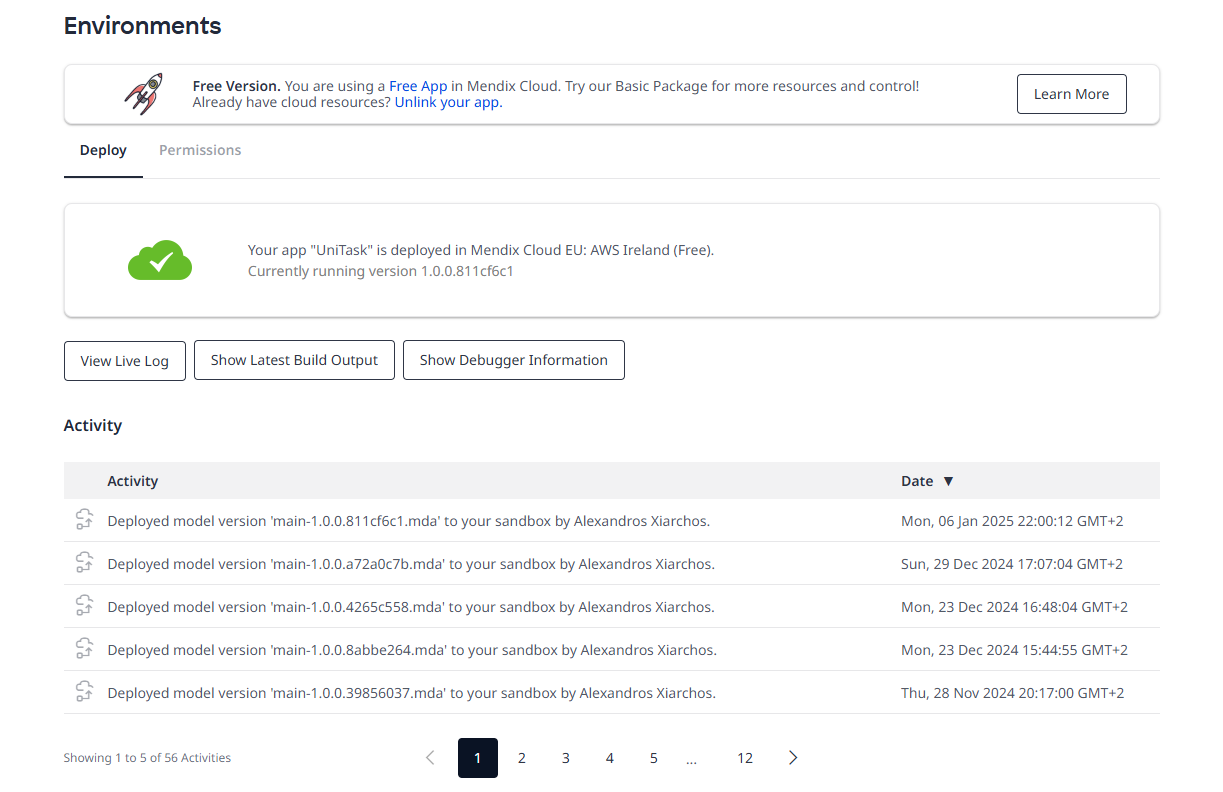
\includegraphics[width=0.9\textwidth]{Mendix/Environments}
                \caption{\centering Σελίδα Environments της εφαρμογής UniTask (κεφ. \ref{ch:unitask})}
                \label{fig:MendixEnvironments}
            \end{figure}


    \section{Δομή εφαρμογών του Mendix}
        Μια εφαρμογή στο Mendix απαρτίζεται από διαφορετικά έγγραφα και modules. Τα modules επιτρέπουν τον διαχωρισμό της εφαρμογής σε αυτόνομα λειτουργικά κομμάτια. Ο τρόπος με τον οποίο πραγματοποιείται ο διαχωρισμός εξαρτάται από την κρίση και τη σχεδιαστική προσέγγιση του μηχανικού λογισμικού.

        \subsection{Modules}
            Μια εφαρμογή αποτελείται από ένα \texttt{App} module, ένα \texttt{System} module, από modules που δημιουργούνται από τους χρήστες, από modules από το marketplace του Mendix ή από modules που καθορίζουν την εμφάνιση της εφαρμογής (UI resources modules). Τα modules του marketplace προσφέρουν έτοιμες λειτουργικότητες κατασκευασμένες από τρίτους ενώ τα UI resources modules εμφανίζονται με πράσινο χρώμα και περιλαμβάνουν πρότυπα σελίδων (page templates) και δομικά στοιχεία (building blocks).

            Για παράδειγμα, στο App Explorer της εφαρμογής RapidDeveloper (εικόνα \ref{fig:MendixStudioOverlay}) παρατηρούμε πως εμφανίζονται τρία διαφορετικά modules: το module \texttt{App}, το module \texttt{System} και το module \texttt{MyFirstModule}. Τα δύο πρώτα είναι modules που δημιουργούνται αυτόματα κατά τη δημιουργία μιας εφαρμογής, ενώ το τρίτο είναι ένα module που δημιουργήθηκε από τον χρήστη.

            Κάθε module περιλαμβάνει ένα domain model, που καθορίζει τη δομή των δεδομένων του. Θα αναφερθούμε αναλυτικά στο domain model στην ενότητα \ref{sec:MendixDomainModel}. Πέρα από το domain models, κάθε module περιλαμβάνει παράθυρα για τις Ρυθμίσεις (Settings) του module και την Ασφάλεια (Security).

            Στις \textbf{Ρυθμίσεις} επιτρέπεται η εξαγωγή του Module ως \textit{App Module} με όλο το πηγαίο κώδικα του ή ως \textit{Add-on Module} με σκοπό να χρησιμοποιηθεί απο άλλους χρήστες, και επίσης εκεί μπορεί να γίνει προσθήκη Java Dependencies στο module. Στην \textbf{Ασφάλεια} μπορεί να καθοριστεί η πρόσβαση όλων των ρόλων χρηστών για κάθε σελίδα, οντότητα ή microflow που υπάρχει στο συγκεκριμένο module.

            \subsubsection{Το module App}
            Κατά τη δημιουργία μιας νέας εφαρμογής, το Mendix παρέχει ένα σύνολο προεγκατεστημένων σελίδων με έτοιμο σχεδιασμό και λειτουργικότητα. Τα αρχεία αυτών των σελίδων βρίσκονται στο module \texttt{App}. Το module \texttt{App} πέρα από τα παράθυρα των Ρυθμίσεων και Ασφάλειας (τα οποία έτσι και αλλιώς υπάρχουν σε όλα τα modules) επιπλέον περιλαμβάνει την Πλοήγηση (Navigation) και τα Κείμενα Συστήματος (System Texts)\footnote{Στο έγγραφο με τα Κείμενα Συστήματος μπορεί να γίνει μετάφραση των μηνυμάτων που παράγονται από τον διακομιστή κατά την εκτέλεση μιας εφαρμογής (για παράδειγμα \say{Password too short}).}. Επιπλέον, περιλαμβάνει ένα φάκελο \texttt{Styling} με \texttt{.js} και \texttt{.css} αρχεία τα οποία χρησιμοποιούνται για το styling της εφαρμογής\footnote{Στα συγκεκριμένα αρχεία μπορούν να επεξεργαστούν μεταβλητές που αφορούν τη σχεδίαση του UI resources module \texttt{Atlas}, το οποίο χρησιμοποιείται ως κεντρικό theme για τις προεγκατεστημένες σελίδες του Mendix. Το \texttt{Atlas} για παράδειγμα περιλαμβάνει έτοιμα color schemes (\texttt{primary}, \texttt{success}, \texttt{warning}, \texttt{danger}, \texttt{info}) τα οποία χρησιμοποιούνται σε όλα τα widgets των σελιδών, όπως επίσης γραμματοσειρές, spacings κτλ. Τα αρχεία λοιπόν αποτελούν έναν από τους τρόπους προσαρμογής της προεπιλεγμένης σχεδίασης του \texttt{Atlas}. Εναλλακτικός τρόπος είναι η δημιουργία ενός custom UI resources module.} και έναν φάκελο \texttt{Marketplace modules} το οποίο περιλαμβάνει εξωτερικά modules που μπορούν να προστεθούν μέσω του Mendix Marketplace.

            Το παράθυρο \textbf{Ρυθμίσεων} του \texttt{App} (εικόνα \ref{fig:MendixAppSettings}) διαφέρει σε σχέση με τα υπόλοιπα modules, καθώς αυτό περιλαμβάνει παραμετροποιήσεις για το runtime περιβάλλον της εφαρμογής, το theme που χρησιμοποιείται, την επιλογή συγκεκριμένων ενεργειών πριν αρχικοποιηθεί η εφαρμογή κατά την εκκίνησή της, επιλογή συγκεκριμένου αλγόριθμου κρυπτογράφησης για το Hashed String τύπο δεδομένων, καθορισμός γλώσσας και άλλα.

            \begin{figure}[h!] \noindent \centering
                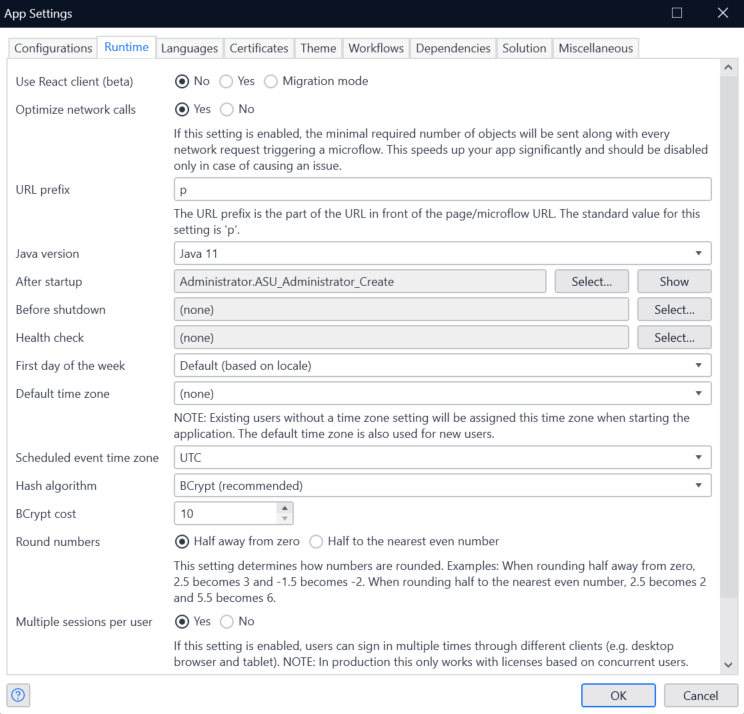
\includegraphics[width=0.7\textwidth]{Mendix/AppSettings}
                \caption{\centering Παράθυρο Settings του App}
                \label{fig:MendixAppSettings}
            \end{figure}

            \begin{figure}[h!] \noindent \centering
                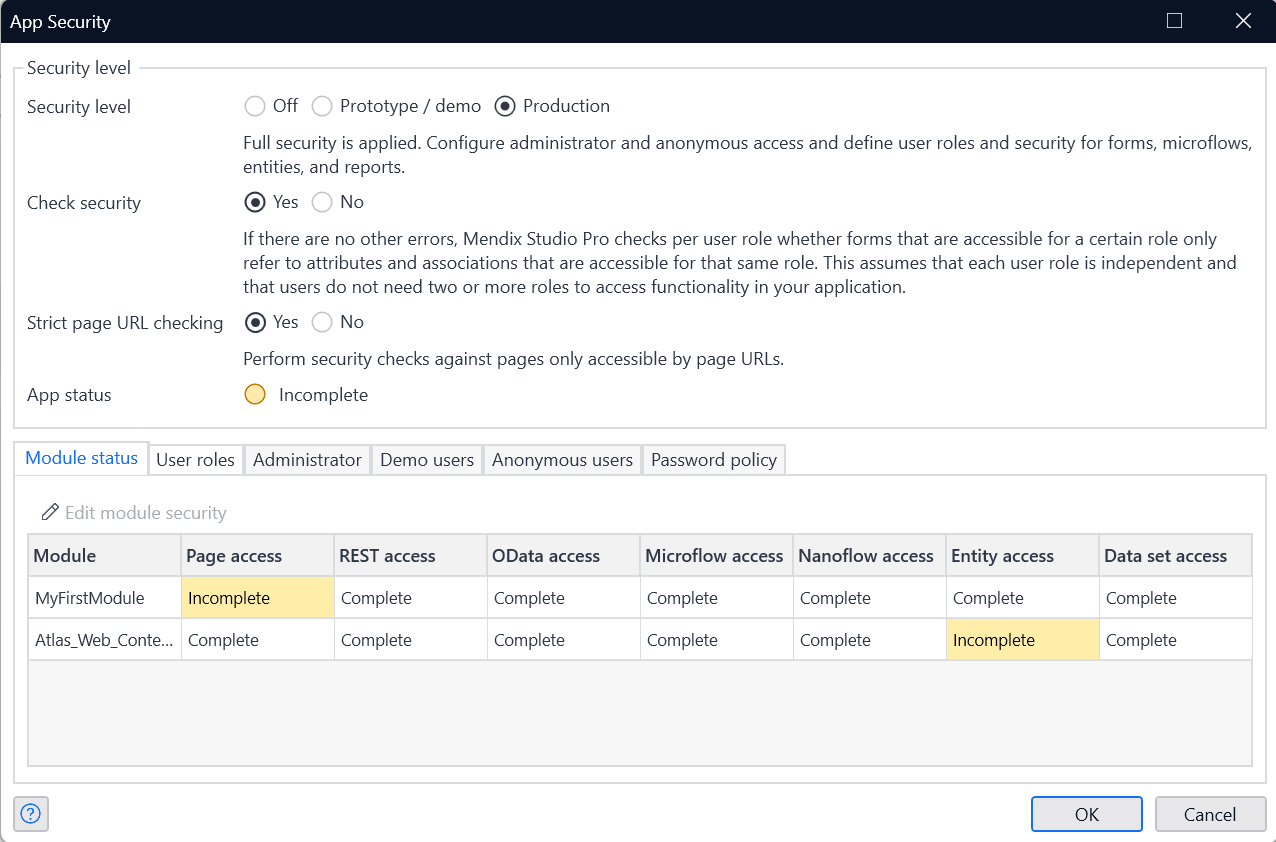
\includegraphics[width=0.8\textwidth]{Mendix/AppSecurity}
                \caption{\centering Παράθυρο Security του App}
                \label{fig:MendixAppSecurity}
            \end{figure}

            Το παράθυρο \textbf{Ασφάλεια} του \texttt{App} (εικόνα \ref{fig:MendixAppSecurity}) το οποίο και αυτό διαφέρει σε σχέση με τα αντίστοιχα παράθυρα των υπόλοιπων modules, χρησιμοποιείται για να τροποποιηθεί το \textit{επίπεδο ασφάλειας} (Security level) της εφαρμογής. Συγκεκριμένα μπορεί να επιλεγεί ώστε οι χρήστες να μη χρειάζεται να συνδεθούν για να έχουν πρόσβαση στην εφαρμογή (Security level = Off), να χρειάζεται να συνδεθούν ώστε να μπορέσουν να χρησιμοποιήσουν φόρμες, microflows κτλ (Security level = Prototype/demo), ή να χρειάζεται να συνδεθούν ώστε να έχουν πρόσβαση στην εφαρμογή καθολικά (Security level = Production).

            Επίσης, μπορούν να οριστούν \textit{ρόλοι χρηστών} όπως για παράδειγμα Administrator, User ή Guest. Κατ' αυτόν τον τρόπο καθίσταται δυνατό να διαχωριστούν τα δικαιώματα πρόσβασης των modules ανάλογα με το ποιος είναι ο ρόλος του χρήστη. Για παράδειγμα, ένας Administrator χρήστης μπορεί να έχει πλήρη πρόσβαση στα modules και στις σελίδες της εφαρμογής, ενώ ένας Guest μπορεί να έχει περιορισμένη προβολή.

            Επιπλέον, στην Ασφάλεια μπορούν να οριστούν τα στοιχεία σύνδεσης του διαχειριστή (Administrator) της εφαρμογής (ώστε να μπορέσει να γίνει η πρώτη σύνδεση κατά το deployment), να οριστούν demo χρήστες (ώστε να δοκιμαστούν οι ρόλοι χρηστών) ή ανώνυμοι χρήστες (οι οποίοι έχουν πρόσβαση στην εφαρμογή χωρίς να συνδεθούν) και να ρυθμιστούν κανόνες για τους κωδικούς πρόσβασης.

            \begin{figure}[h!] \noindent \centering
                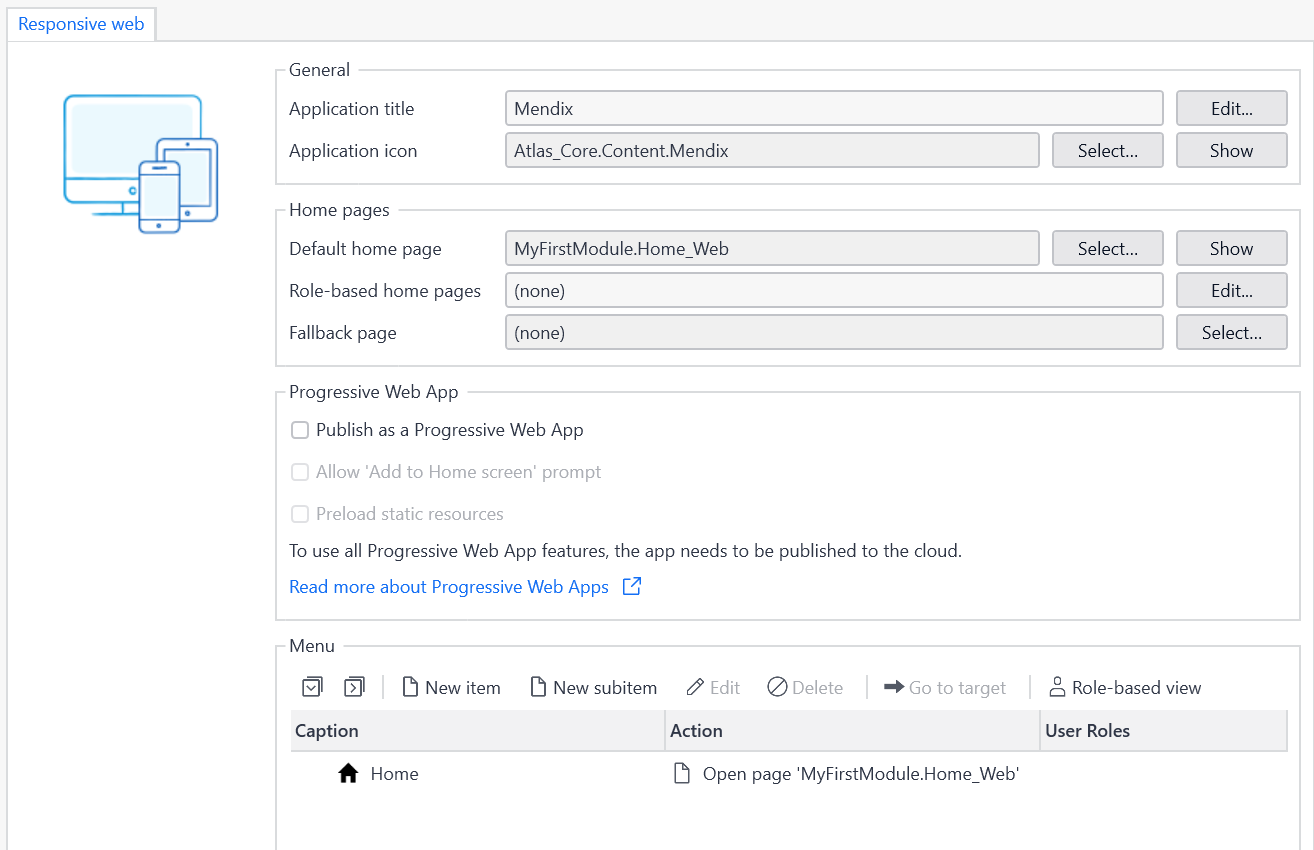
\includegraphics[width=0.8\textwidth]{Mendix/Navigation}
                \caption{\centering Το έγγραφο Navigation}
                \label{fig:MendixAppNavigation}
            \end{figure}

            Η \textbf{Πλοήγηση} του module \texttt{App} (εικόνα \ref{fig:MendixAppNavigation}) εμφανίζει το σύνολο των σελίδων του κεντρικού μενού της εφαρμογής. Εκεί μπορεί να γίνει η επεξεργασία του μενού με την προσθήκη στοιχείων ή και υποστοιχείων σε στοιχεία. Επίσης, περιλαμβάνονται διαφορετικές προβολές ανάλογα με τον εκάστοτε ρόλο χρήστη, στις οποίες εμφανίζονται μόνο οι σελίδες που είναι προσβάσιμες σε κάθε ρόλο. Στην Πλοήγηση επίσης μπορεί να διαμορφωθεί το όνομα και το εικονίδιο της εφαρμογής, καθώς και να οριστεί η αρχική σελίδα (home page) της, η οποία μάλιστα μπορεί να διαμορφωθεί ώστε να είναι διαφορετική για τον εκάστοτε ρόλο χρήστη \cite{mendixDoc}.

            \subsubsection{Το module System}
                Το module \texttt{System} είναι ένα προεγκατεστημένο module που περιλαμβάνει τη βασική λειτουργικότητα η οποία χρησιμοποιείται στις ήδη κατασκευασμένες σελίδες και microflows του \texttt{App}. Το συγκεκριμένο module δεν μπορεί να επεξεργαστεί από τον χρήστη, αλλά μπορούν με βάσει αυτό να προστεθούν συσχετίσεις (associations) ή γενικεύσεις (generalizations) τα modules τα οποία κατασκευάζονται από τους χρήστες. Για παράδειγμα, μπορεί να δημιουργηθεί μια οντότητα \texttt{Πελάτης} η οποία θα συσχετίζεται με την οντότητα \texttt{User} του module \texttt{System} και έτσι θα κληρονομεί τις ρυθμίσεις ασφαλείας του \cite{mendixSystemModule}.

        \subsection{Έγγραφα}
            Η Πλοήγηση είναι ένα \textit{έγγραφο} της εφαρμογής. Άλλα παραδείγματα εγγράφων είναι οι \textit{Σελίδες} (Pages) (βλ. ενότητα \ref{sec:MendixPages}), τα \textit{Microflows} (βλ. ενότητα \ref{sec:MendixMicroflows}) και τα \textit{Enumerations}\footnote{Τα enumerations (κατάλογος, απαρίθμηση) καθορίζουν μια λίστα από προκαθορισμένες τιμές. Για παράδειγμα, ένα enumeration μπορεί να χρησιμοποιηθεί για τον καθορισμό της κατάστασης μιας εργασίας ως \texttt{To do}, \texttt{Done} ή \texttt{Doing}.}.

        \subsection{Σελίδες} \label{sec:MendixPages}
            Η σελίδα είναι ο κεντρικός τρόπος αλληλεπίδρασης του χρήστη με την εφαρμογή. Η δημιουργία μιας σελίδας μπορεί να βασιστεί σε \textit{πόρους} που προέρχονται από έγγραφα, όπως οι Εικόνες (Images), τα Layouts τα οποία καθορίζουν τη διάταξη της σελίδας, τα Μενού (Menus) που διαμορφώνουν την πλοήγηση, ή τα Snippets, τα οποία αποτελούν επαναχρησιμοποιήσιμα τμήματα διεπαφής.\footnote{Το Mendix είναι μια Εφαρμογή Μίας Σελίδας (Single-page application -- SPA) που σημαίνει ότι όλη η αλληλεπίδραση πραγματοποιείται σε μία μόνο καρτέλα ή παράθυρο του προγράμματος περιήγησης που φορτώνεται μία φορά και στη συνέχεια ενημερώνεται δυναμικά χωρίς να χρειάζεται να φορτωθεί ξανά. Ως αποτέλεσμα, δεν είναι δυνατό το άνοιγμα νέων σελίδων σε διαφορετική καρτέλα ή παράθυρο.}

                \begin{figure}[h!] \noindent \centering
                    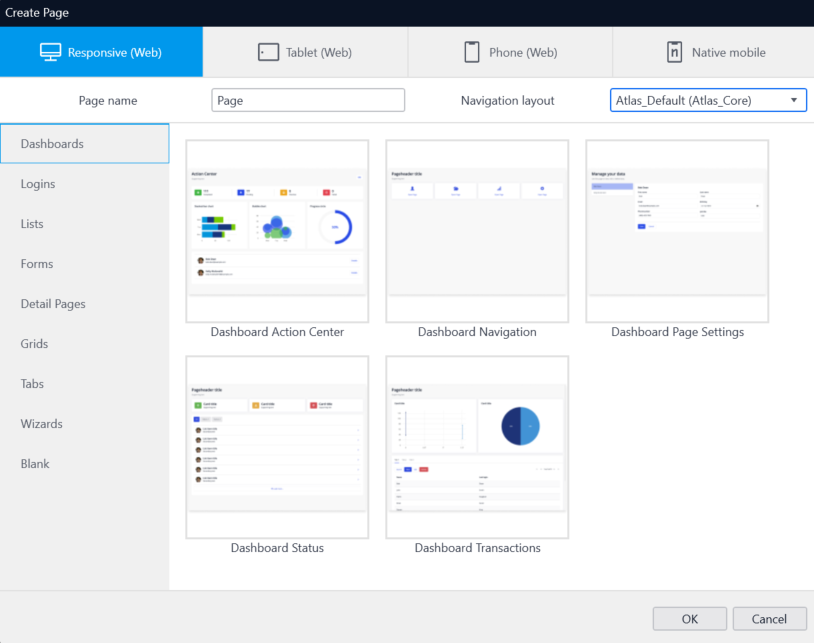
\includegraphics[width=0.7\textwidth]{Mendix/CreateNewPage}
                    \caption{\centering Το παράθυρο δημιουργίας μιας νέας σελίδας}
                    \label{fig:MendixCreateNewPage}
                \end{figure}

            \subsubsection{Layout}
            Κάθε σελίδα στο Mendix βασίζεται σε ένα προκαθορισμένο layout, το οποίο καθορίζει βασικές ιδιότητες της σελίδας, όπως το μήκος, το πλάτος ή για παράδειγμα αν πρόκειται για αναδυόμενη (popup) σελίδα. Επιπλέον, τα layouts επιτρέπουν τον ορισμό στατικών τμημάτων, όπως ένα header ή ένα μενού, που παραμένουν σταθερά σε όλες τις σελίδες που τα χρησιμοποιούν. Για παράδειγμα, θα μπορούσαν να δημιουργηθούν δύο layouts όπου το ένα θα έχει το μενού πλοήγησης ως μπάρα στο πάνω μέρος της οθόνης και το άλλο κάθετη στα αριστερά. Το Mendix προσφέρει επίσης προκαθορισμένα πρότυπα σελίδων (page templates), τα οποία διευκολύνουν τη γρήγορη και απλή δημιουργία σελίδων με προκαθορισμένη δομή και σχεδίαση.

            Η εικόνα \ref{fig:MendixCreateNewPage} απεικονίζει το παράθυρο δημιουργίας νέας σελίδας, όπου ο χρήστης μπορεί να επιλέξει είτε από τα έτοιμα πρότυπα είτε να δημιουργήσει μια κενή σελίδα. Εδώ δίνεται επίσης η δυνατότητα επιλογής του layout (Navigation layout) της σελίδας, το οποίο μπορεί να είναι είτε ένα από τα προεγκατεστημένα layouts του Mendix είτε ένα προσαρμοσμένο layout που έχει δημιουργηθεί από τον χρήστη.

            \subsubsection{Widgets}
                Τα Widgets είναι προδιαμορφωμένα στοιχεία, έτοιμες λειτουργικές μονάδες που μπορούν να προστεθούν απευθείας σε κάθε σελίδα της εφαρμογής. Πρόκειται για εργαλεία που ενσωματώνονται εύκολα μέσω του Toolbox, όπως παρουσιάστηκε στην εικόνα \ref{fig:MendixStudioOverlay}. Ενδεικτικά παραδείγματα περιλαμβάνουν:

                \begin{itemize}[label={\tiny \blacksquare}]
                    \setlength\itemsep{-0.25em}
                    \item \textbf{Data containers} -- δομές δεδομένων που περιέχουν δεδομένα από τη βάση δεδομένων. Παραδείγματα είναι Data view, Data grid, List view κ.α.
                    \item \textbf{Text widgets} -- περιέχουν κείμενο. Παραδείγματα είναι Text, Label, Page Title κ.α.
                    \item \textbf{Structure widgets} -- δομικά στοιχεία που χρησιμοποιούνται για την οργάνωση των widgets στη σελίδα. Παραδείγματα είναι Layout grid, Container, Tab container, Snippet call, Table κ.α.
                    \item \textbf{Input widgets} -- πεδία εισόδου δεδομένων. Παραδείγματα είναι Text box, Text area, Check box, Radio button, Drop-down, Date picker, File uploader κ.α.
                    \item \textbf{Images, Videos ή Files} -- widgets που περιέχουν πολυμέσα.
                    \item \textbf{Buttons} -- widgets που εκτελούν ενέργειες. Το Mendix παρέχει αρκετά buttons με προκαθορισμένες ενέργειες για την εκτέλεση ενεργειών όπως Save, Cancel, Delete, New, Edit, Crate, Call microflow κ.α.
                \end{itemize}

            \begin{figure}[h!] \noindent \centering
                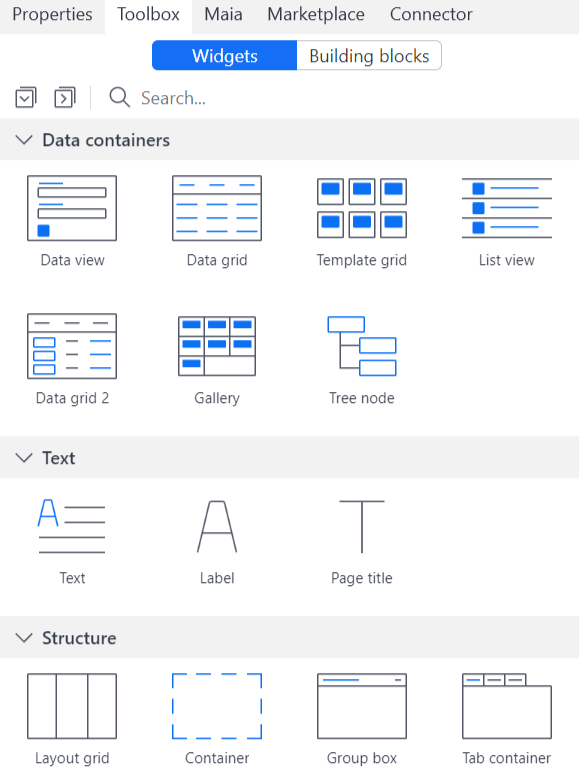
\includegraphics[width=0.4\textwidth]{Mendix/ToolboxPage}
                \caption{\centering Τα Widgets περιλαμβάνονται στο Toolbox panel}
                \label{fig:MendixToolboxPage}
            \end{figure}

                Tο Mendix προσφέρει προκαθορισμένα σύνολα από widgets (εικόνα \ref{fig:MendixToolboxPage}), γνωστά ως \textit{Building blocks}, τα οποία δημιουργούν στοιχεία όπως επικεφαλίδες (headers), φόρμες και ειδοποιήσεις (notifications). Αυτά τα Building blocks διευκολύνουν και επιταχύνουν τη διαδικασία ανάπτυξης, παρέχοντας στους χρήστες έτοιμες λύσεις που μπορούν να ενσωματωθούν απευθείας στις εφαρμογές.

                \begin{figure}[h!] \noindent \centering
                    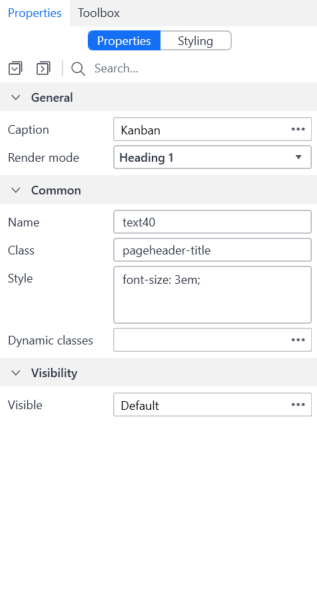
\includegraphics[width=0.3\textwidth]{Mendix/PropertiesPanel1}
                    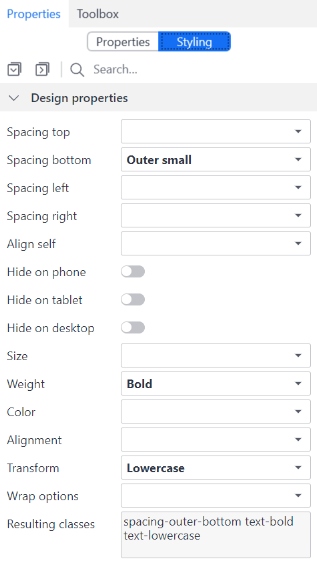
\includegraphics[width=0.3\textwidth]{Mendix/PropertiesPanel2}
                    \caption{\centering Το panel Properties}
                    \label{fig:MendixPropertiesPanel}
                \end{figure}

                Τέλος, για κάθε widget (όπως και για κάθε σελίδα) μπορούν να επεξεργαστούν οι ιδιότητές του. Το panel Properties (εικόνα \ref{fig:MendixPropertiesPanel}) είναι ένα δυναμικό panel το οποίο αλλάζει το περιεχόμενό του ανάλογα με το στοιχείο που έχουμε επιλεγμένο. Στο Properties μπορούμε να ορίσουμε συνθήκες όπου θα επιτρέπεται η εμφάνιση ενός στοιχείου, να επιλέξουμε διαφορετικά render styles από τα προδιαμορφωμένα που παρέχει το Mendix, να ορίσουμε events που θα συμβαίνουν όταν ο χρήστης αλληλεπιδρά με το στοιχείο, όπως επίσης και να αλλάξουμε CSS κλάσεις είτε μέσω των παρεχόμενων επιλογών του Mendix είτε μέσω της προσθήκης δικού μας custom CSS κώδικα.

        \subsubsection{Εμφάνιση σελίδων} \label{sec:MendixPageView}
            Το Mendix Studio Pro επιτρέπει την προβολή μιας σελίδας είτε σε Structure Mode είτε σε Design Mode, παρέχοντας διαφορετικές οπτικές για τη διαχείριση και τον σχεδιασμό της.

            \begin{figure}[h!] \noindent \centering
                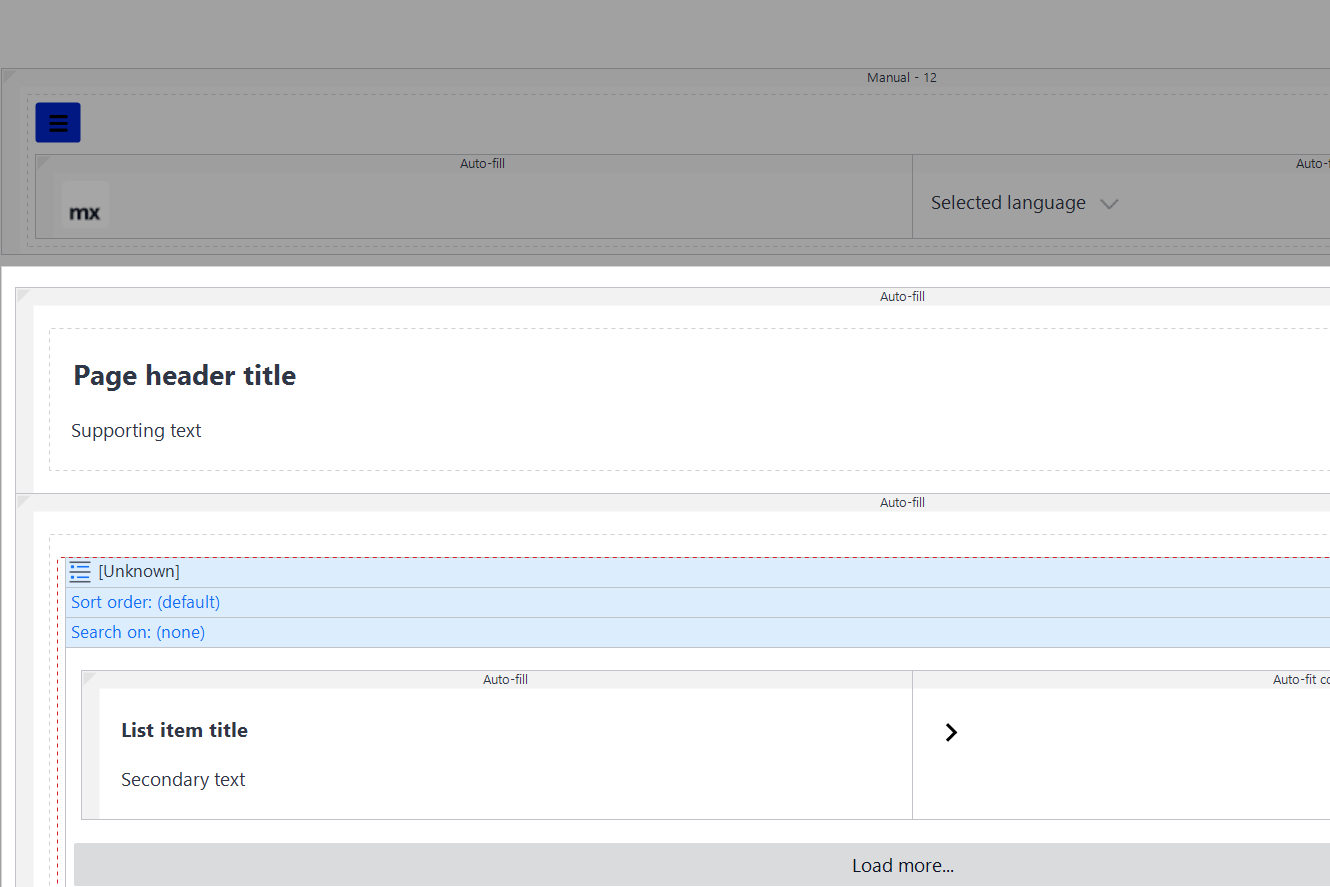
\includegraphics[width=0.6\textwidth]{Mendix/PageView2} \\
                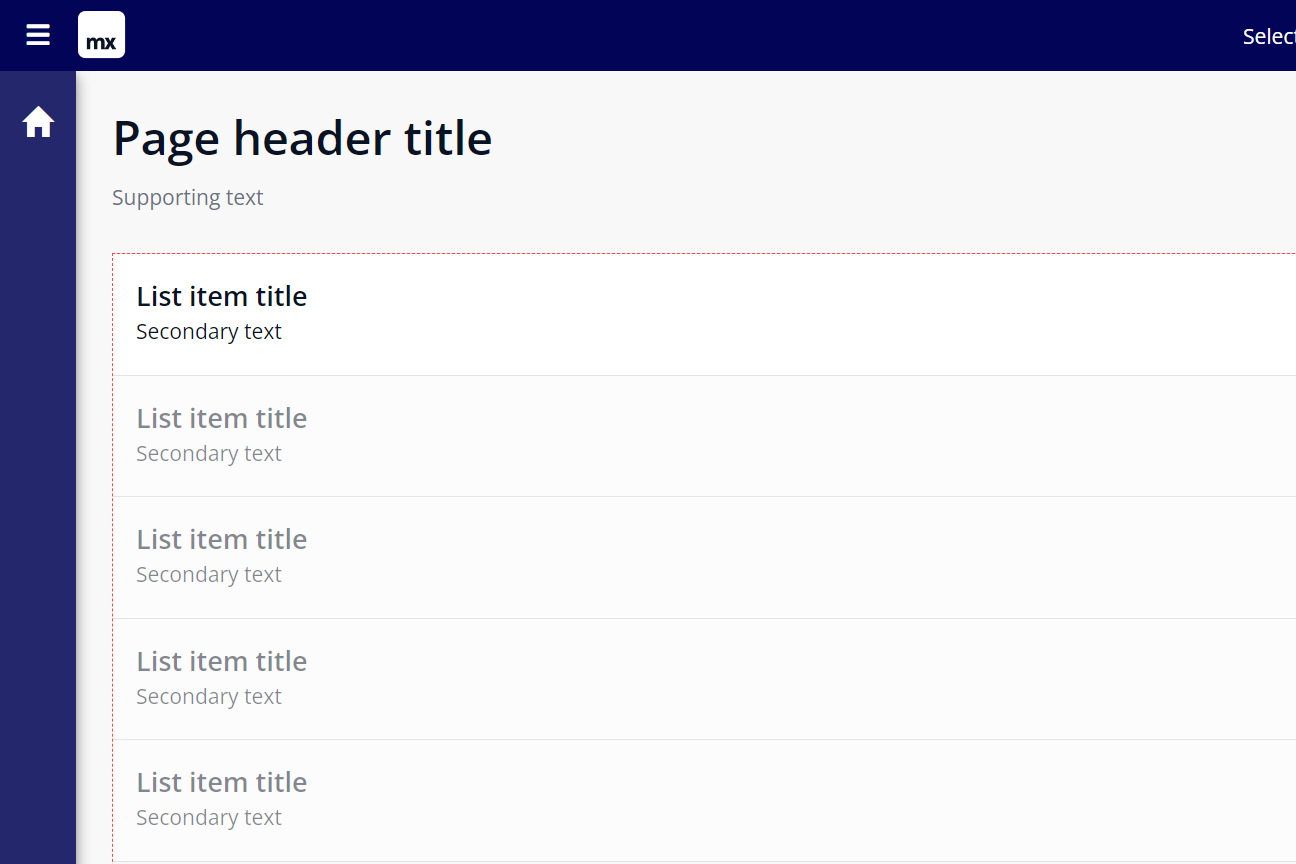
\includegraphics[width=0.6\textwidth]{Mendix/PageView1} \\
                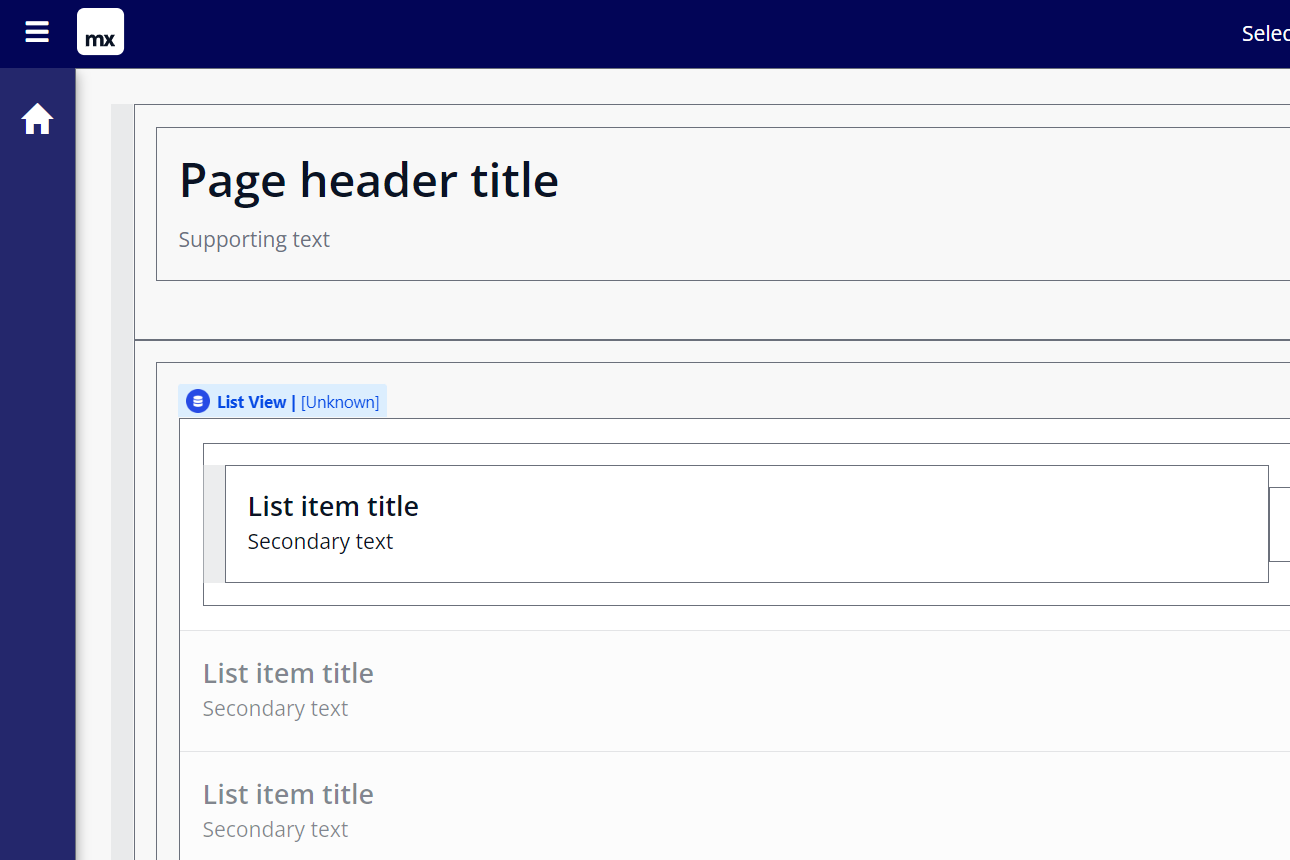
\includegraphics[width=0.6\textwidth]{Mendix/PageView3}
                \caption{\centering Διαφορετικές εμφανίσεις της ίδιας σελίδας από αριστερά \\ προς τα δεξιά: Structure Mode, Design Mode, X-Ray Mode.}
            \end{figure}

            Στο \textbf{Structure Mode}, παρουσιάζονται με σαφήνεια όλα τα δομικά στοιχεία που συνθέτουν τη σελίδα, δίνοντας έμφαση στη δομή της και επιτρέποντας την εύκολη προσαρμογή και οργάνωση των περιεχομένων. Αυτή η λειτουργία είναι ιδανική για την ανάλυση της λογικής της σελίδας, τη διαχείριση των στοιχείων της και τη διόρθωση πιθανών προβλημάτων διάταξης. Είναι επίσης ο μοναδικός τρόπος προβολής των εφαρμογών κινητών συσκευών (Native mobile).

            Αντίθετα, στο \textbf{Design Mode}, η σελίδα απεικονίζεται όπως ακριβώς θα εμφανίζεται στον τελικό χρήστη. Αυτό προσφέρει μια πιο ρεαλιστική απεικόνιση της εμπειρίας χρήστη. Επιπλέον, το Design Mode περιλαμβάνει τη λειτουργία \textbf{X-Ray Mode}, η οποία συνδυάζει στοιχεία από το Structure Mode και το Design Mode. Με το X-Ray Mode, οι χρήστες μπορούν να δουν τόσο την αισθητική εμφάνιση όσο και τη δομή της σελίδας ταυτόχρονα. Αυτή η λειτουργία επιτρέπει την ακριβή τοποθέτηση και διαχείριση στοιχείων, ενώ ταυτόχρονα προσφέρει τη δυνατότητα άμεσων προσαρμογών σε επίπεδο σχεδιασμού και λογικής.

            Οι διαφορετικές προβολές μπορούν να επιλεγούν από το πάνω μέρος του Working Area, το οποίο επιπλέον περιλαμβάνει και δυνατότητα αλλαγών στο μέγεθος του καμβά της σελίδας ώστε να ελεγχθεί το πως εμφανίζεται η εφαρμογή σε κινητά και τάμπλετ.

        \subsubsection{Παράδειγμα δομής σελίδας}
            \begin{figure}[h!] \noindent \centering
                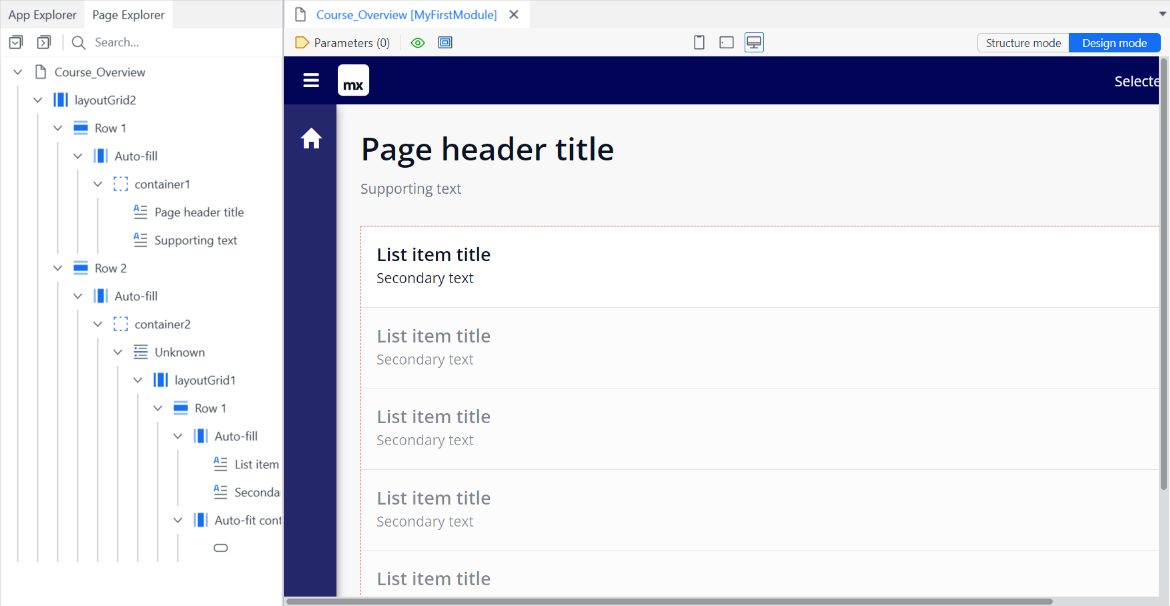
\includegraphics[width=\textwidth]{Mendix/PageExplorer}
                \caption{\centering Page Explorer και Working area της σελίδας \texttt{Course\_Overview}}
                \label{fig:MendixPageExplorer}
            \end{figure}

            Στην εικόνα \ref{fig:MendixPageExplorer} εμφανίζεται o Page Explorer και το Working area της σελίδας \verb|Course_Overview| της εφαρμογής RapidDeveloper. Παρατηρούμε πως όλη η σελίδα είναι δομημένη γύρω από ένα Layout Grid, το οποίο αποτελείται από δύο Rows (γραμμές). Το \texttt{Row 1} δημιουργεί το Header της σελίδας μαζί με το Supporting text τα οποία είναι τοποθετημένα σε ένα container\footnote{Τα containers διευκολύνουν την ομαδοποίηση κοινών στοιχείων της σελίδας, επιτρέποντας την εύκολη εφαρμογή κανόνων, όπως ο έλεγχος της ορατότητας (visibility), συγκεκριμένων events ή και custom CSS κλάσεις.}, και το \Texttt{Row 2} δημιουργεί ένα List View το οποίο επαναλαμβάνεται. Το List View αποτελείται και αυτό από ένα Layout Grid το οποίο δημιουργεί τα δύο texts τα οποία βλέπουμε στη λίστα όπως επίσης και ένα κουμπί (το οποίο εμφανίζεται εκτός οθόνης). Η μπλε οριζόντια μπάρα και η μπλε κάθετη μπάρα στα αριστερά αποτελούν κομμάτι του Layout της σελίδας, το οποίο είναι το \verb|Atlas_Default|.


        \subsection{Microflows} \label{sec:MendixMicroflows}
            Τα Microflows (όπως και τα Nanoflows και τα Workflows)\footnote{Η βασική διαφορά μεταξύ Microflows και Nanoflows έγκειται στη λειτουργικότητα και τον τρόπο εκτέλεσής τους. Τα Microflows βασίζονται σε βιβλιοθήκες της Java, εκτελούνται στον διακομιστή (runtime server) και, ως εκ τούτου, δεν είναι διαθέσιμα για εφαρμογές που λειτουργούν εκτός σύνδεσης. Από την άλλη πλευρά, τα Nanoflows χρησιμοποιούν βιβλιοθήκες της JavaScript, εκτελούνται στην πλευρά του client, γεγονός που τα καθιστά εν δυνάμει γρηγορότερα.

            Τα Microflows είναι ιδανικά για την προσκόμιση και την επεξεργασία δεδομένων από τη βάση δεδομένων ή από εξωτερικές πηγές, εξασφαλίζοντας υψηλή αξιοπιστία και συνέπεια. Αντίθετα, τα Nanoflows χρησιμοποιούνται κυρίως για ενέργειες που σχετίζονται με την εμπειρία του χρήστη, όπως η εμφάνιση αναδυόμενων (pop-up) μηνυμάτων, η προβολή progress bars ή η ανταλλαγή cookies.

            Τέλος, τα Workflows ενδείκνυνται για τη διαχείριση σταθερών και επαναλαμβανόμενων διαδικασιών, επιτρέποντας την αυτοματοποίηση και την απλοποίηση της εκτέλεσής τους.} συνιστούν τον βασικό μηχανισμό εκτέλεσης λογικής στις εφαρμογές του Mendix καθώς αναπαριστούν τη λογική της εφαρμογής με έναν οπτικό τρόπο χαμηλού κώδικα. Αυτά τα διαγράμματα ροής (εικόνα \ref{fig:MendixMicroflowExample}) απεικονίζουν τη λογική εκτέλεσης διαφόρων εντολών και αλληλουχιών ενεργειών, επιτρέποντας την κατασκευή σύνθετης λειτουργικότητας χωρίς την ανάγκη γραφής παραδοσιακού κώδικα. Χρησιμοποιούνται ευρέως για ενέργειες όπως η δημιουργία, η ενημέρωση και η διαγραφή δεδομένων, η εμφάνιση σελίδων, το φιλτράρισμα δεδομένων, η εκτέλεση ελέγχων, η είσοδος δεδομένων από εξωτερικές πηγές και άλλα.

            \begin{figure}[h!] \noindent \centering
                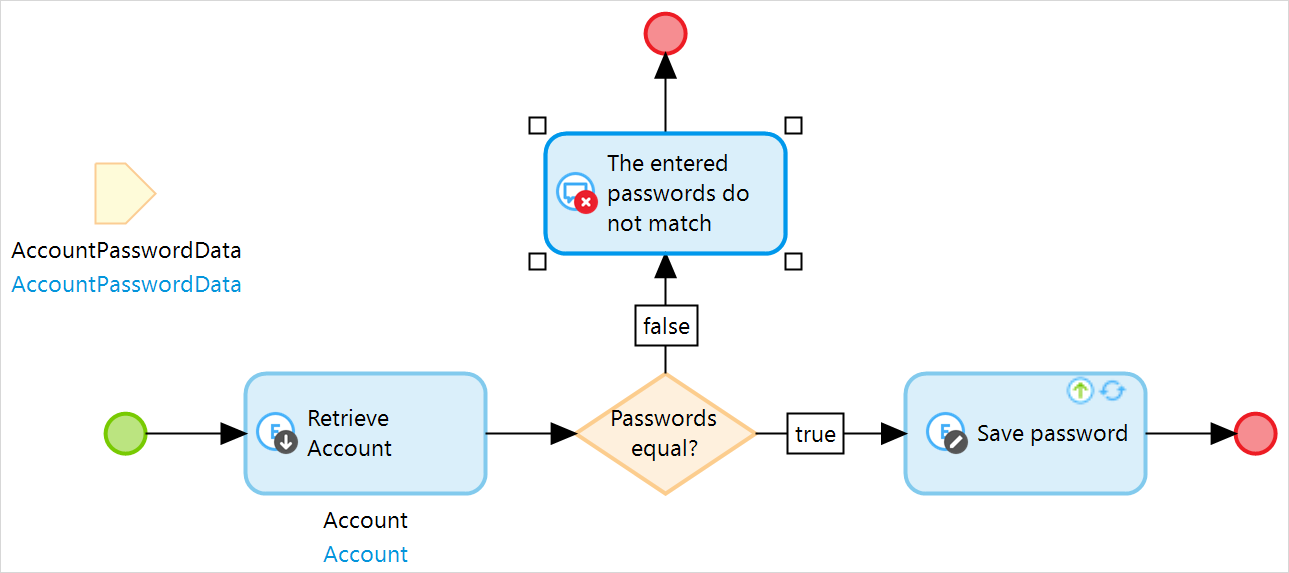
\includegraphics[width=0.7\textwidth]{Mendix/microflow-nanoflow-example}
                \caption{\centering Παράδειγμα Microflow. Τα πράσινα και κόκκινα κυκλάκια αναπαριστούν τα events, τα μπλε ορθογώνια τα activities και ο πορτοκαλί ρόμβος το decision. Ως είσοδο έχουμε το parameter AccountPasswordData \cite{mendixDoc}.}
                \label{fig:MendixMicroflowExample}
            \end{figure}

            Τα Microflows αποτελούνται από τα παρακάτω στοιχεία:
                \begin{itemize}[label={\tiny \blacksquare}]
                    \setlength\itemsep{-0.25em}
                    \item \textbf{Events} -- λειτουργούν ως σημεία εκκίνησης και τερματισμού του Microflow. Χρησιμοποιώντας το τελικό event μπορούμε να ορίσουμε την τιμή και το τύπο δεδομένων που επιστρέφει το Microflow, με παρόμοιο τρόπο όπως στις συναρτήσεις ή μεθόδους του υψηλού κώδικα.
                    \item \textbf{Decisions} -- επιτρέπουν την εισαγωγή λογικών συνθηκών. Για παράδειγμα, ένα decision μπορεί να ελέγξει αν μια μεταβλητή έχει τιμή και, ανάλογα με την απάντηση, να κατευθύνει τη ροή σε διαφορετικές ενέργειες. Οι συνθήκες ορίζονται με τη χρήση εκφράσεων (βλ. ενότητα \ref{sec:MendixExpressions}).
                    \item \textbf{Activities} -- αποτελούν τις κύριες ενέργειες που εκτελούνται στη ροή. Παραδείγματα τέτοιων ενεργειών είναι η δημιουργία (ή ενημέρωση ή διαγραφή) αντικειμένων μέσω του activity Create (ή Change ή Delete) object, η εμφάνιση μιας σελίδας στον χρήστη μέσω του Show page, η κλήση ενός άλλου Microflow μέσω του Microflow call, το φιλτράρισμα λιστών (List operation), η σύνδεση με εξωτερικές υπηρεσίες μέσω REST APIs κ.α.
                    \item \textbf{Loops} -- επιτρέπουν την εκτέλεση επαναλαμβανόμενων ενεργειών.
                    \item \textbf{Parameter} -- πρόκειται για τα δεδομένα εισόδου του Microflow, με αντίστοιχη λογική όπως οι συναρτήσεις υψηλού κώδικα.
                \end{itemize}

            \begin{figure}[h!] \noindent \centering
                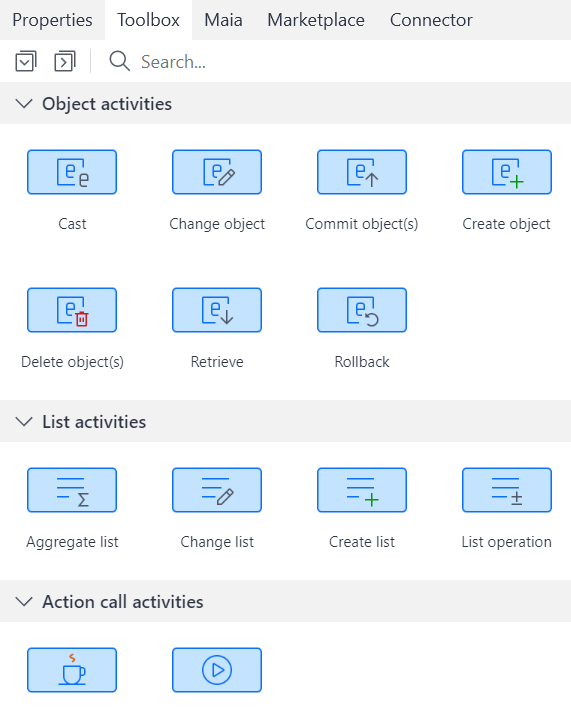
\includegraphics[width=0.4\textwidth]{Mendix/ToolboxMicroflow}
                \caption{\centering Όταν επεξεργαζόμαστε ένα Microflow, \\ τo Toolbox panel περιλαμβάνει τα διαθέσιμα activities.}
            \end{figure}

            Ένα Microflow μπορεί να εκτελεστεί από διαφορετικά μέρη όπως το Navigation menu, ένα κουμπί, ένα link ή ακόμα και να καλεστεί από ένα άλλο Microflow. Επιπλέον, τα Microflows μπορούν να εκτελεστούν αυτόματα μετά από μια συγκεκριμένη ενέργεια (Event Handlers), όπως η αποθήκευση ενός αντικειμένου ή η ενημέρωση ενός πεδίου.

            Τέλος, κάθε Microflow αποθηκεύεται ως ένα Java αρχείο στον πηγαίο κώδικα της εφαρμογής. Για εξειδικευμένες λειτουργίες, το Mendix παρέχει τη δυνατότητα ενσωμάτωσης προσαρμοσμένου κώδικα Java μέσω του $ \text{App} \rightarrow \text{Deploy to Eclipse} $.

        \subsection{Εκφράσεις} \label{sec:MendixExpressions}
            Οι εκφράσεις (expressions) του Mendix είναι ένας τρόπος ενσωμάτωσης λειτουργικότητας στην εφαρμογή μας. Οι εκφράσεις μπορούν να περιλαμβάνουν σταθερές τιμές, μεταβλητές, συναρτήσεις, λογικές πράξεις, συγκρίσεις, επιλογές κ.α. Για παράδειγμα, μπορεί να οριστεί η εμφάνιση ενός συγκεκριμένου widget μόνο αν ισχύει μια συγκεκριμένη συνθήκη. Οι εκφράσεις μπορούν να χρησιμοποιηθούν σε πολλά σημεία της εφαρμογής, όπως στα Microflows, στις ιδιότητες των widgets κ.α.

            Για παράδειγμα, η έκφραση \verb|if $package/weight < 1.00 then 0.00 else 5.00| ελέγχει το γνώρισμα \texttt{weight} της οντότητας \texttt{package} και επιστρέφει \texttt{0.00} αν το βάρος είναι μικρότερο από \texttt{1.00}, αλλιώς επιστρέφει \texttt{5.00}. Θα δούμε περισσότερες τέτοιες εκφράσεις στην πράξη στο κεφάλαιο \ref{ch:unitask}.

        \subsection{Domain Model} \label{sec:MendixDomainModel}
            Το domain model αναπαριστά τη δομή των δεδομένων κάποιου module στην πλατφόρμα Mendix. Τα δεδομένα που περιγράφονται από το domain model αποθηκεύονται στη συνέχεια σε ένα σχεσιακό σύστημα βάσεων δεδομένων του Mendix.

            Το domain model αποτελεί κεντρικό πυλώνα της αρχιτεκτονικής κάθε εφαρμογής. Κάθε module έχει το δικό του domain model, και όλα τα modules μπορούν να χρησιμοποιούν δεδομένα από όλα τα υπόλοιπα domain modules μέσω συσχετίσεων.

            \begin{figure}[h!] \noindent \centering
                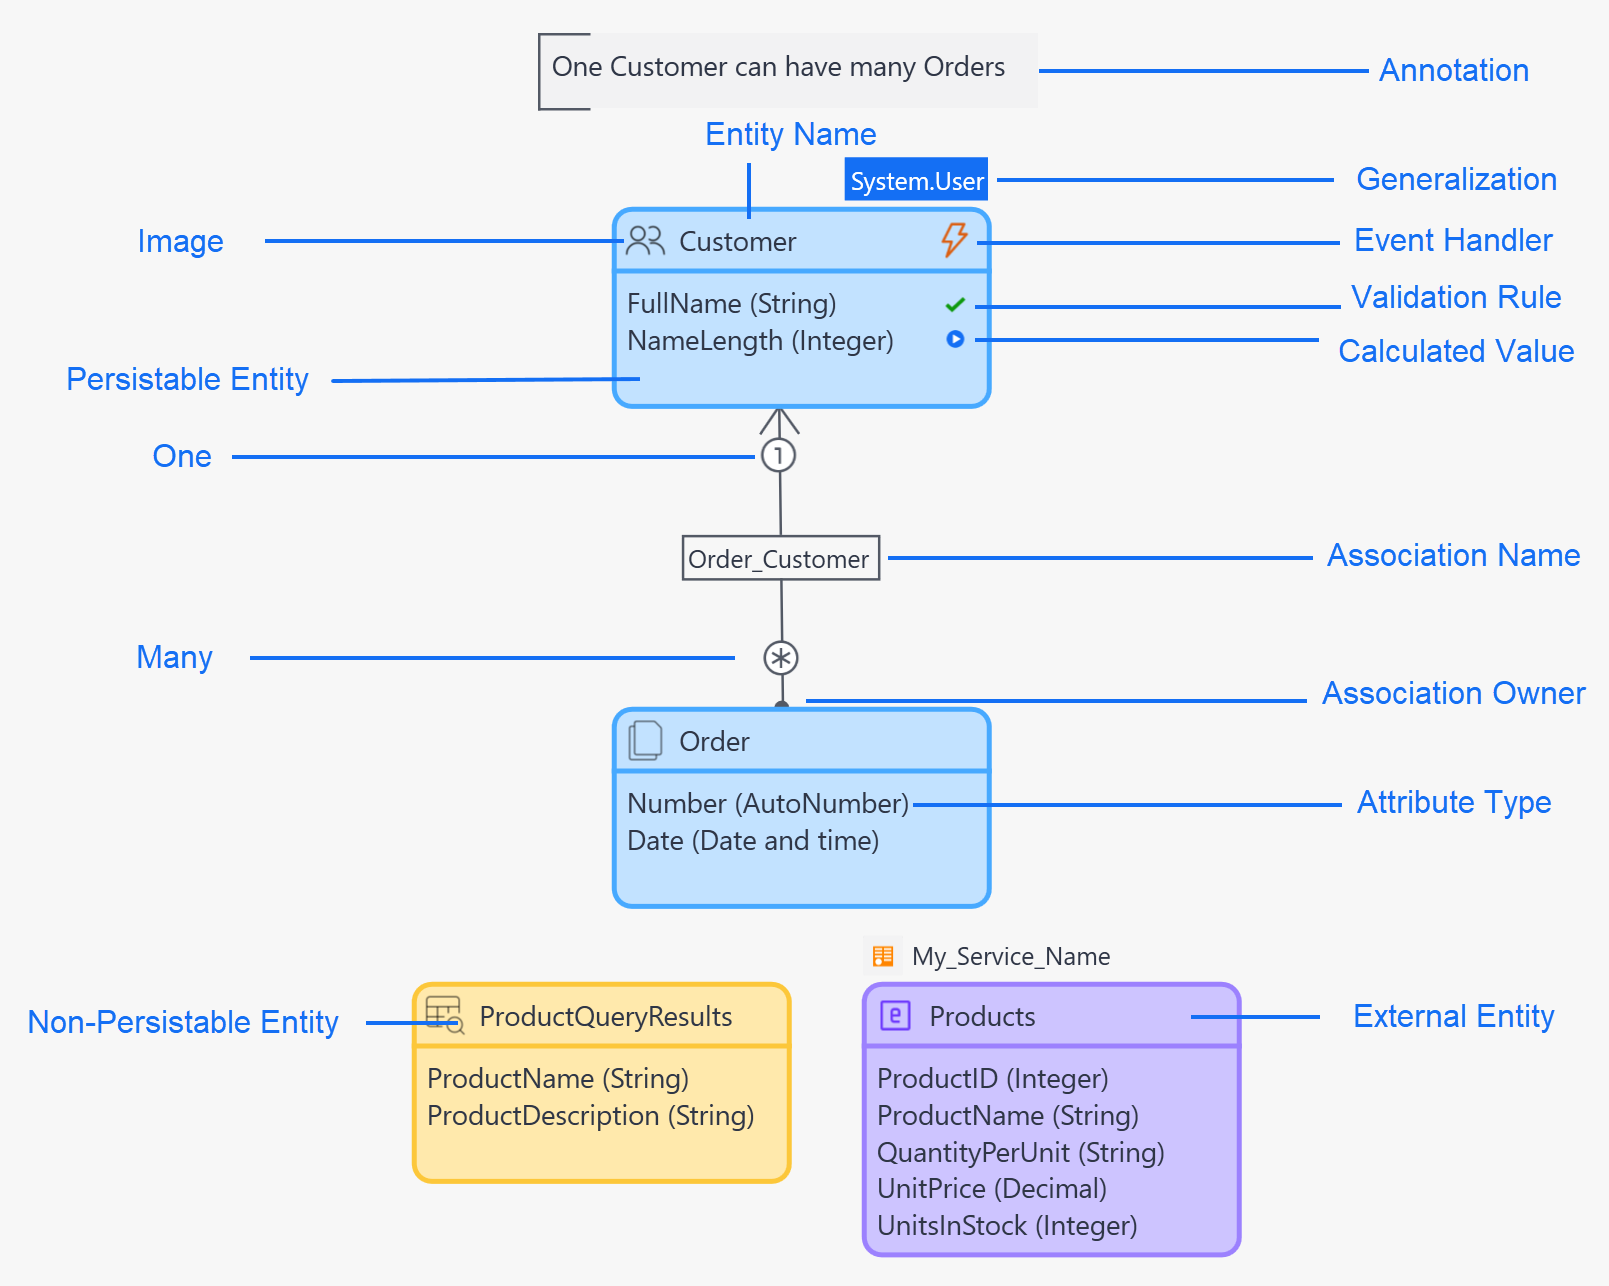
\includegraphics[width=0.8\textwidth]{Mendix/annotated-domain-model}
                \caption{\centering Παράδειγμα από domain model \cite{mendixDoc}}
                \label{fig:MendixDomainModel}
            \end{figure}

            Η εικόνα \ref{fig:MendixDomainModel} είναι ένα παράδειγμα ενός domain model που αναπαριστά πελάτες και παραγγελίες. Οι πελάτες και οι παραγγελίες αποτελούν οντότητες (entities) του domain model. Οι οντότητες συσχετίζονται μεταξύ τους με μια συσχέτιση (association) πολλών-προς-ένα. Κάθε παραγγελία ανήκει σε έναν μόνο πελάτη, ενώ ένας πελάτης μπορεί να σχετίζεται με πολλές παραγγελίες. Φυσικά, το Mendix περιλαμβάνει και άλλες πληθικότητες, όπως συσχετίσεις ένα-προς-ένα όπως επίσης και πολλά-προς-πολλά. Επιπλέον, αν διαγραφτεί κάποια οντότητα μπορεί να ρυθμιστεί τι θα συμβεί με τις συσχετίσεις της (π.χ. να διαγραφούν και αυτές).

            Μέσα στα ορθογώνια που αναπαριστούν τις οντότητες βρίσκονται τα γνωρίσματα, οι ιδιότητες (attributes) των οντοτήτων. Στην παρένθεση κάθε γνωρίσματος καταγράφεται ο τύπος δεδομένων του. Παρατηρούμε πως υπάρχουν ορθογώνια με διαφορετικά χρώματα, κάτι που αντιστοιχεί σε διαφορετικού είδους οντότητες. Τα μπλε ορθογώνια αναπαριστούν οντότητες που αποθηκεύονται στη βάση δεδομένων, με κίτρινο μη-διατηρήσιμες οντότητες (non-persistent entities), δηλαδή οντότητες που δεν αποθηκεύονται στη βάση δεδομένων αλλά αποθηκεύονται προσωρινά στη μνήμη, και τέλος με μωβ οντότητες από εξωτερικές πηγές δεδομένων. Η μπλε ετικέτα \texttt{System.User} που συνοδεύει την οντότητα \texttt{Customer} δηλώνει πως η οντότητα αυτή βασίζεται σε μια άλλη οντότητα, την οντότητα \texttt{User} του module \texttt{System} (Γενίκευση -- Generalization)\footnote{Η έννοια της γενίκευσης στο Mendix βασίζεται σε μια λογική που θυμίζει την κληρονομικότητα (inheritance) στις αντικειμενοστραφείς γλώσσες προγραμματισμού, δηλαδή επιτρέπει σε μία οντότητα (entity) να κληρονομεί τις ιδιότητες και τις συσχετίσεις μιας άλλης υπεροντότητας, χρησιμοποιώντας τα χαρακτηριστικά και τις συσχετίσεις της, ενώ παράλληλα μπορεί να ορίσει πρόσθετες ιδιότητες ή συσχετίσεις που είναι μοναδικές για την ίδια. Η γενίκευση είναι ιδιαίτερα χρήσιμη καθώς συμβάλλει στη διατήρηση της ακεραιότητας και της ασφάλειας των δεδομένων. Για παράδειγμα, οι \say{Customers} που κληρονομούν τα γνωρίσματα της οντότητας \texttt{System.User}, ταυτόχρονα κληρονομούν και όλα τα χαρακτηριστικά ασφάλειας του \texttt{User} που το Mendix έχει προδιαμορφώσει.}. Τέλος, ανάλογα αν στην οντότητα έχει οριστεί κάποιος Event handler ή αν σε κάποιο γνώρισμα υπάρχει κάποιο validation rule, το Mendix το αναγνωρίζει και το αναπαριστά με το αντίστοιχο σύμβολο.

            \subsubsection{Οντότητες}
                \begin{figure}[h!] \noindent \centering
                    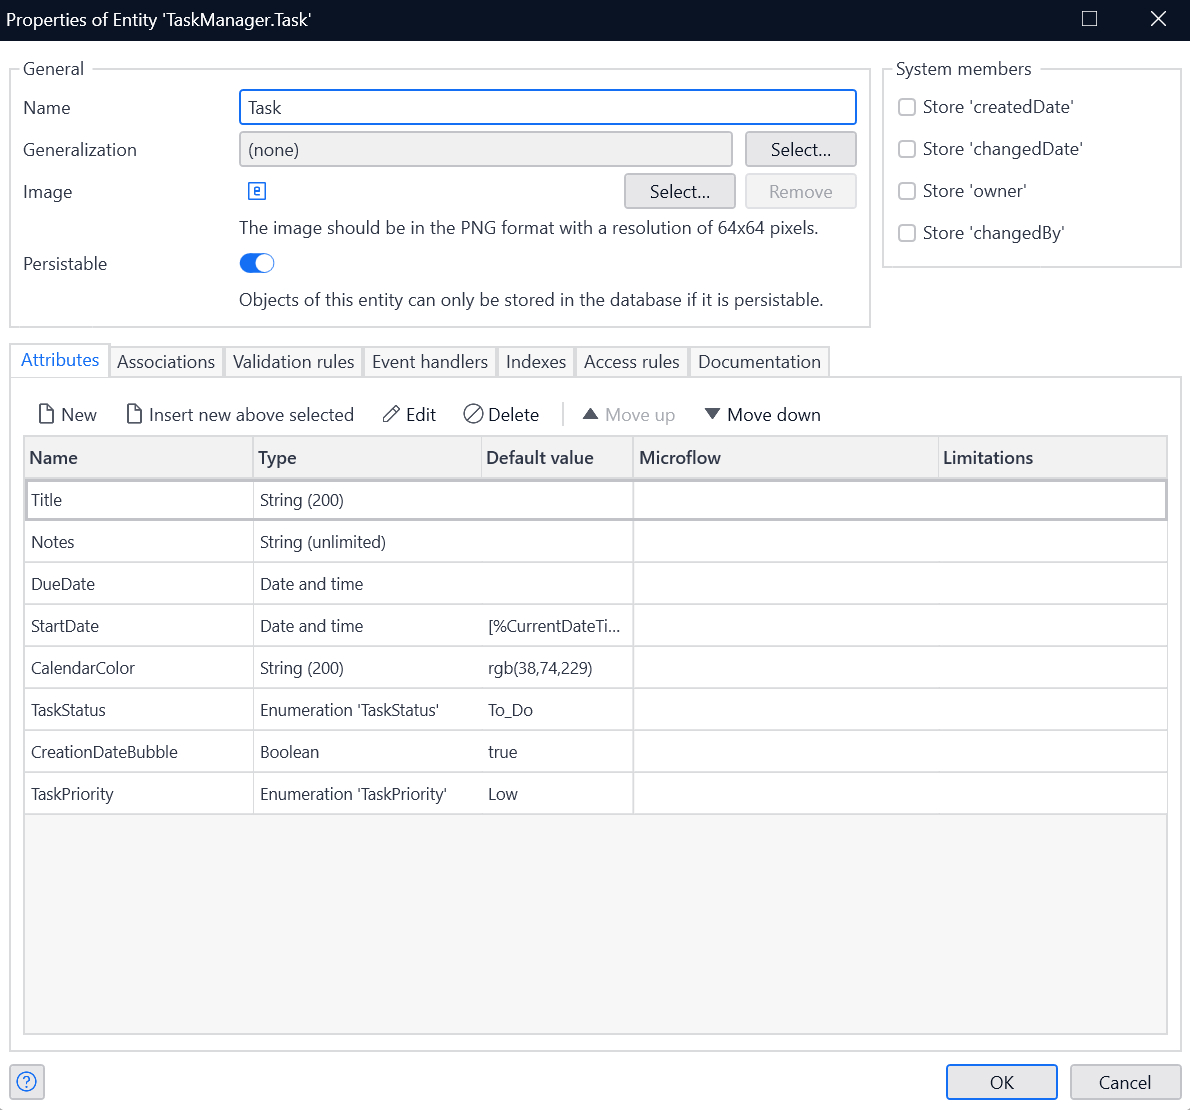
\includegraphics[width=0.7\textwidth]{Mendix/EntityProperties}
                    \caption{\centering Ιδιότητες μιας οντότητας Task (βλ. κεφ. \ref{ch:unitask})}
                    \label{fig:MendixEntityProperties}
                \end{figure}

                Στην εικόνα \ref{fig:MendixEntityProperties} παρουσιάζεται το παράθυρο που εμφανίζεται όταν δημιουργούμε ή επεξεργαζόμαστε μια οντότητα. Στο πάνω μέρος ορίζεται αν η οντότητα έχει κάποια γενίκευση και το αν είναι διατηρήσιμη στη βάση δεδομένων.

                Στην καρτέλα \textbf{Attributes} (Γνωρίσματα) καθορίζονται όλα τα γνωρίσματα της οντότητας. Εκεί επιλέγεται ο τύπος δεδομένων του γνωρίσματος. Οι τύποι δεδομένων που υποστηρίζονται από το Mendix είναι οι εξής: \texttt{AutoNumber} (αυτόματα παραγόμενοι αριθμοί, π.χ. IDs), \texttt{Binary}, \texttt{Boolean}, \texttt{Date and time}, \texttt{Decimal}, \texttt{Enumeration} (επιλέγεται κάποιο Enumeration έγγραφο), \texttt{Hashed string}, \texttt{Integer}, \texttt{Long}, \texttt{String}. Ο τύπος ενός γνωρίσματος είναι πιθανό να καθοριστεί αυτόματα από το Mendix βάσει του ονόματος που επιλέγεται κατά τον ορισμό του. Τέλος, μπορεί να οριστεί μια προεπιλεγμένη τιμή του κάθε ορίσματος ή να οριστεί η τιμή να καθορίζεται από κάποιο microflow.

                \begin{figure}[h!] \noindent \centering
                    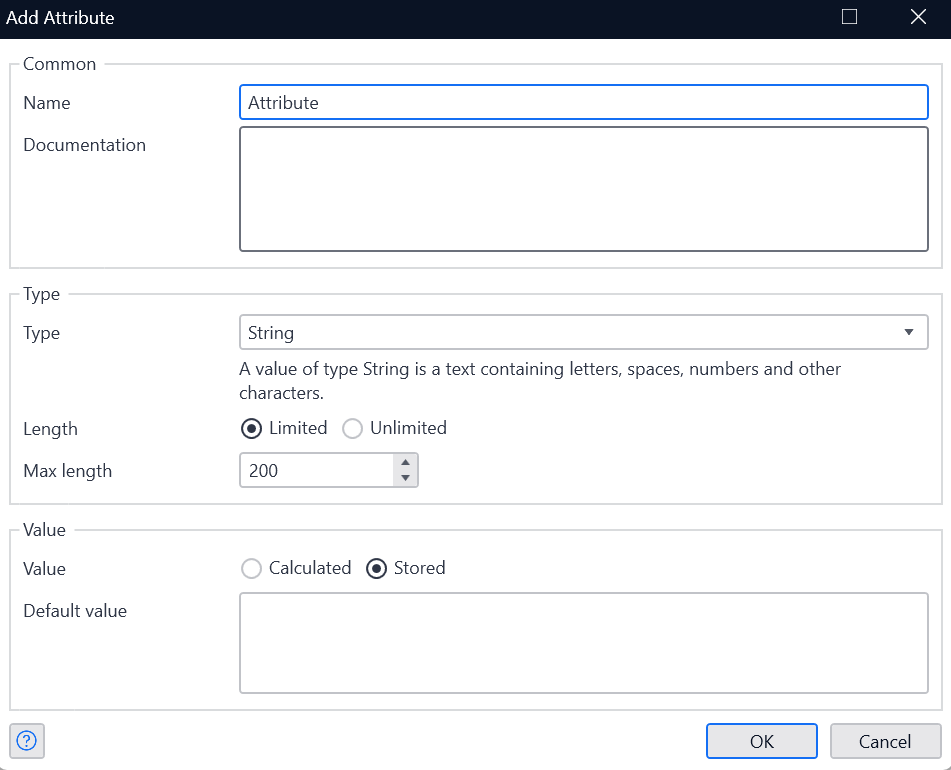
\includegraphics[width=0.6\textwidth]{Mendix/AddAttribute}
                    \caption{\centering Προσθήκη καινούριου γνωρίσματος σε μια οντότητα}
                \end{figure}

                Η καρτέλα \textbf{Associations} (Συσχετίσεις) είναι ένας τρόπος επεξεργασίας των συσχετίσεων μιας οντότητας. Ένας εναλλακτικός τρόπος είναι απευθείας από το domain model μέσω των συνδέσεων μεταξύ των οντοτήτων.

                \begin{figure}[h!] \noindent \centering
                    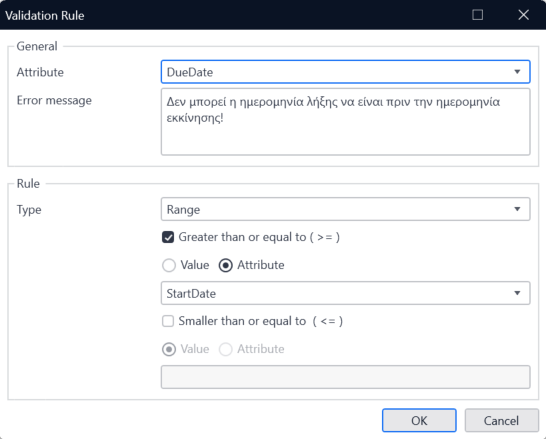
\includegraphics[width=0.6\textwidth]{Mendix/ValidationRule}
                    \caption{\centering Προσθήκη κανόνα επικύρωσης (βλ. κεφ. \ref{ch:unitask})}
                \end{figure}

                \begin{figure}[h!] \noindent \centering
                    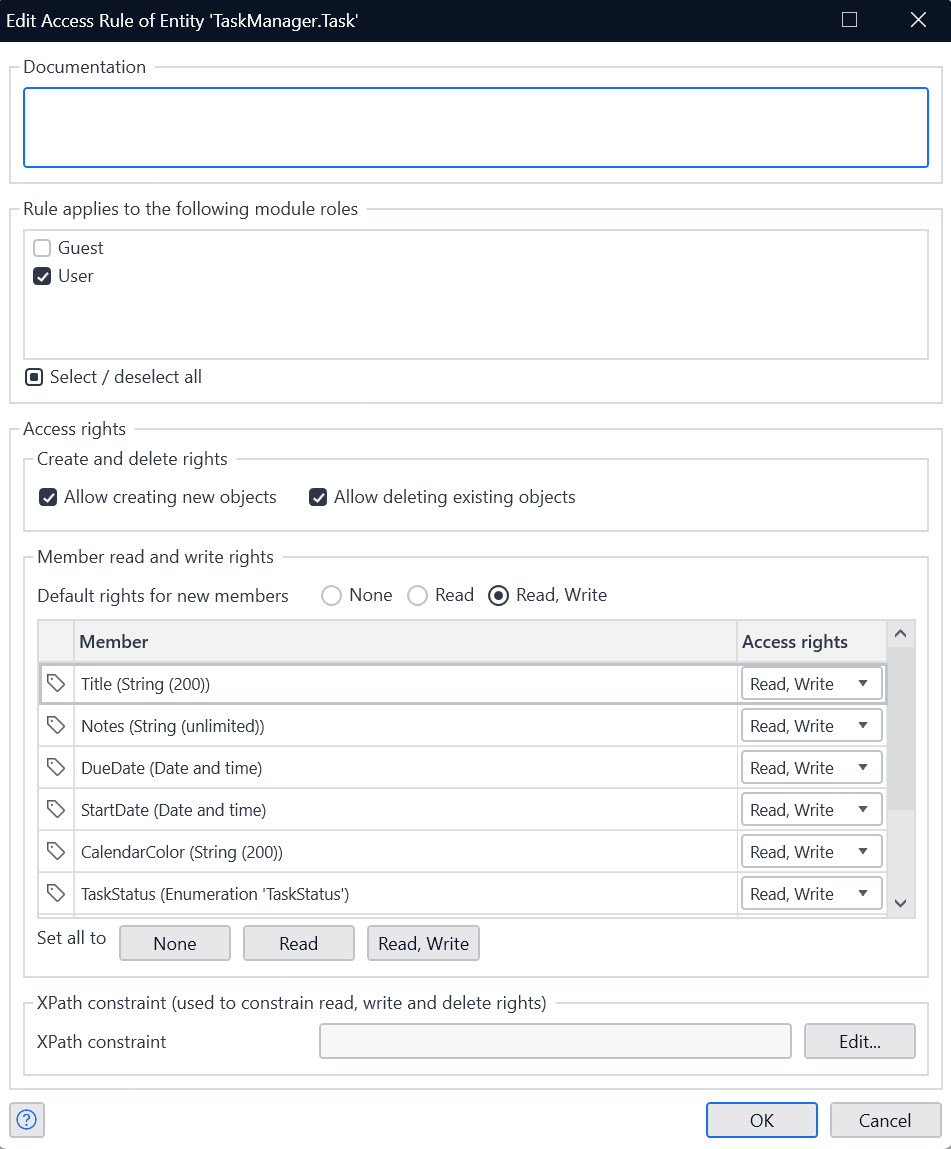
\includegraphics[width=0.62\textwidth]{Mendix/AccessRuleEntity}
                    \caption{\centering Επεξεργασία κανόνων πρόσβασης της οντότητας Task (βλ. κεφ. \ref{ch:unitask})}
                \end{figure}

                Η καρτέλα \textbf{Validation rules} (Κανόνες Επικύρωσης) δημιουργεί συνθήκες που πρέπει να ικανοποιούνται για να είναι έγκυρα τα γνωρίσματα κάθε οντότητας. Οι κανόνες επικύρωσης μπορούν να είναι απλές συνθήκες, όπως π.χ. ένα πεδίο να μην είναι κενό, ή πιο σύνθετες, όπως π.χ. η τιμή ενός πεδίου να καθορίζεται από ένα εύρος τιμών. Αν η συνθήκη δεν πληρούται, εμφανίζεται αυτόματα μήνυμα σφάλματος κάτω από το πεδίο.

                Η καρτέλα \textbf{Event handlers} (Χειριστές Συμβάντων) είναι ένας τρόπος για να εκτελεστούν συγκεκριμένες ενέργειες (microflows) όταν συμβεί κάποιο συγκεκριμένο συμβάν στην οντότητα. Τα συμβάντα μπορεί να είναι η δημιουργία (create), η ενημέρωση (commit ή save), η διαγραφή (delete) ή η ακύρωση (rollback ή cancel) μιας οντότητας. Μπορεί να επιλεγεί η εκτέλεση του microflow πριν ή μετά την εκτέλεση των παραπάνω συμβάντων.

                Η καρτέλα \textbf{Access Rules} (Κανόνες Πρόσβασης) ορίζει τα δικαιώματα κάθε ρόλου χρήστη όσον αφορά την αλληλεπίδραση με τα γνωρίσματα της οντότητας. Μπορεί να επιλεγεί ποιος ρόλος χρήστη μπορεί να δημιουργήσει ή να διαγράψει στιγμιότυπα από οντότητες και να διαβάσει ή να τροποποιήσει τα γνωρίσματά τους.

                Τέλος, μπορούν να προστεθούν breakpoints στα Microflows ώστε να εντοπιστούν σφάλματα μέσω debugging κατά την εκτέλεσή τους.

            \subsection{Dashboard εφαρμογής}
                Παράλληλα με την ανάπτυξη της εφαρμογής στο Mendix Studio Pro, στο προσωπικό προφίλ κάθε χρήστη υπάρχει ένα dashboard για κάθε εφαρμογή που αναπτύσσουμε όπου παρέχονται project management εργαλεία και μεθοδολογίες ανάπτυξης λογισμικού.

                \begin{figure}[h!] \noindent \centering
                    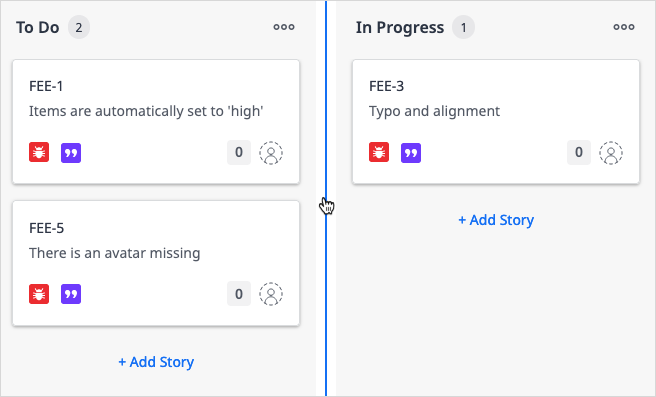
\includegraphics[width=0.5\textwidth]{Mendix/Scrum}
                    \caption{\centering Πίνακας Kanban στο dashboard \cite{mendixDoc}}
                \end{figure}
